\documentclass[10pt, a4paper]{article}

% Page
\usepackage{pdflscape} % make certain pages landscape
\usepackage{geometry} % set page geometry
\usepackage[indent=2em, skip=0.8em plus 0.1 em minus 0.2 em]{parskip} % set paragraph spacing

% Font and Text
\usepackage[utf8]{inputenc}
\usepackage{bbm} % blackboard bold fonts
\usepackage{lmodern} % bold teletype font
\usepackage{csquotes} % allows quoting blocks of text
\usepackage{textcomp} % allow text settings
\usepackage{xcolor} % allows for colouring of source code blocks
\usepackage{url} % better URLs
\usepackage{indentfirst} % indent the first line after a heading
\usepackage{enumitem} % gives alphabet list headers

% Notation
\usepackage{amssymb} % allows for maths mode symbols
\usepackage{amsmath} % allows for many maths mode commands
\usepackage{amsthm} % allows for QED tombstone
\usepackage{mathtools}
\allowdisplaybreaks% allow display elements to break across pages
\usepackage{siunitx} % allows SI units to be formatted
\usepackage{braket} % support Dirac notation
\usepackage{esvect} % nicer vector arrows
\usepackage[thinc]{esdiff} % derivatives 
\usepackage{esint} % integrals
\usepackage{cancel} % allow cancellation

% Tables
\usepackage{tabulary} % allows for better tables
\usepackage{longtable} % allows tables to span pages
\usepackage{makecell} % allow nice table titles
\usepackage[export]{adjustbox} % allow tables to take up the space they need, and export additional scaling stuff for graphicx
\usepackage{diagbox} % diagonal box in table
\usepackage{multirow} % cells in tables can span rows/columns
\usepackage{tablefootnote} % use \tablefootnote for footnotes in tables

% Code
\usepackage{listings} % allows for source code blocks
\usepackage{algorithm} % typeset algorithms
\usepackage{algpseudocode} % pseudocode style algorithms

% Document
\usepackage[backend=biber, style=ieee]{biblatex}
\addbibresource{../wiring.bib}
\graphicspath{{../images/}}
\usepackage{appendix}
\usepackage{hyperref} % hyperlinks
\usepackage{bookmark} % PDF bookmarks
\hypersetup{%
  colorlinks=true,
  linkcolor=purple,
  urlcolor=blue
}
\usepackage{cleveref} % references are automatically of the form "Section 1" etc.
\Crefname{subsection}{Subsection}{Subsections}
\AtBeginEnvironment{appendices}{\crefalias{section}{appendix}}

\numberwithin{equation}{section} % eqn counter rolls over at each section
\newcounter{stmt} % definitions, theorems and lemmas share this counter

\theoremstyle{definition}
\newtheorem{defn}[stmt]{Definition}
\theoremstyle{plain}
\newtheorem{question}{Question}
\newtheorem{funqn}{Fundamental Question}
\newtheorem{theorem}[stmt]{Theorem}
\newtheorem{lemma}[stmt]{Lemma}

% Custom lengths
\addtolength{\jot}{0.5em} % gives spacing between align* rows

\newenvironment{Tabular}[1] % less cramped tables
{\def\arraystretch{1.75}\begin{tabular}{#1}}
{\end{tabular}}
\newenvironment{Array*}[1] % less cramped display mode arrays
{\def\arraystretch{1.75}\everymath={\displaystyle}\[\begin{array}{#1}}
{\end{array}\]}
\newenvironment{Array}[1] % less cramped display mode arrays
{\def\arraystretch{1.75}\everymath={\displaystyle}\begin{equation}\begin{array}{#1}}
{\end{array}\end{equation}}
\newenvironment{displaytable}[1] % environment for a simple inline table to present some information
{\vspace\abovedisplayskip\begin{center}\begin{tabular}{#1}}
{\end{tabular}\end{center}\vspace\belowdisplayskip}

\newcommand{\tableline}[1]{\dimexpr \linewidth/#1 - 2\tabcolsep}

% temporarily change margins
\newenvironment{changemargin}[2]{% 
  \begin{list}{}{%
      \setlength{\topsep}{0pt}%
      \setlength{\leftmargin}{#1}%
      \setlength{\rightmargin}{#2}%
      \setlength{\listparindent}{\parindent}%
      \setlength{\itemindent}{\parindent}%
      \setlength{\parsep}{\parskip}%
    }%
\item[]}{\end{list}}

  % Graphics
  \usepackage[justification=centering]{caption} % centres captions
  \usepackage{float} % stop LaTeX from making stuff float everywhere with H
  \usepackage{graphicx} % allows figures to be inserted and scaled
  \usepackage{tikz} % programmatically draw stuff
  \usepackage{tikzscale} % include .tikz files with includegraphics and scale them
  \usetikzlibrary{shapes, shapes.geometric, automata, positioning, arrows}

  \RequirePackage{luatex85}
  % Default preamble
  \usepackage{pgfplots}
  \pgfplotsset{compat=newest}
  \usepgfplotslibrary{groupplots}
  \usepgfplotslibrary{polar}
  \usepgfplotslibrary{smithchart}
  \usepgfplotslibrary{statistics}
  \usepgfplotslibrary{dateplot}
  \usepgfplotslibrary{ternary}
  \usetikzlibrary{arrows.meta}
  \usetikzlibrary{backgrounds}
  \usepgfplotslibrary{patchplots}
  \usepgfplotslibrary{fillbetween}
  \pgfplotsset{%
    layers/standard/.define layer set={%
      background,axis background,axis grid,axis ticks,axis lines,axis tick labels,pre main,main,axis descriptions,axis foreground%
      }{grid style= {/pgfplots/on layer=axis grid},%
      tick style= {/pgfplots/on layer=axis ticks},%
      axis line style= {/pgfplots/on layer=axis lines},%
      label style= {/pgfplots/on layer=axis descriptions},%
      legend style= {/pgfplots/on layer=axis descriptions},%
      title style= {/pgfplots/on layer=axis descriptions},%
      colorbar style= {/pgfplots/on layer=axis descriptions},%
      ticklabel style= {/pgfplots/on layer=axis tick labels},%
      axis background@ style={/pgfplots/on layer=axis background},%
      3d box foreground style={/pgfplots/on layer=axis foreground},%
    },
  }

  \tikzset{%
    ->, % makes the edges directed
    >=stealth, % makes the arrow heads bold
    node distance=3cm, % specifies the minimum distance between two nodes. Change if necessary.
    every state/.style={thick, fill=gray!10}, % sets the properties for each ’state’ node
    initial text=$ $, % sets the text that appears on the start arrow
  }

  \definecolor{codegreen}{rgb}{0,0.6,0}
  \definecolor{codered}{rgb}{0.6,0,0}
  \definecolor{codeblue}{rgb}{0,0,0.6}
  \definecolor{codepurple}{rgb}{0.58,0,0.82}
  \definecolor{backcolour}{rgb}{0.95,0.95,0.95}

  \lstset{%
    numbers=left,                   % where to put the line-numbers
    stepnumber=1,                   % the step between two line-numbers.        
    numbersep=5pt,                  % how far the line-numbers are from the code
    backgroundcolor=\color{white},  % choose the background color. You must add \usepackage{color}
    showspaces=false,               % show spaces adding particular underscores
    showstringspaces=false,         % underline spaces within strings
    showtabs=false,                 % show tabs within strings adding particular underscores
    tabsize=2,                      % sets default tabsize to 2 spaces
    captionpos=b,                   % sets the caption-position to bottom
    breaklines=true,                % sets automatic line breaking
    % breakatwhitespace=true,         % sets if automatic breaks should only happen at whitespace
    upquote=true, 			% set all single quotes to straight quotes
    basicstyle={\ttfamily\small},           % hackerman teletype font
    keywordstyle={\color{codegreen}\bfseries\ttfamily}, % hackerman teletype font
    commentstyle={\color{codeblue}\textit},           % fancy italic comments
    stringstyle={\color{codered}},           % string literal highlighting
    identifierstyle={}, 
    %title=\lstname,                % show the filename of files included with \lstinputlisting;
    frame=single,			% put a frame around the source code
    aboveskip=2em, % add space before code
    inputpath={./code/}
  }

  % analysis and calculus
  \DeclareMathOperator*{\argmin}{argmin}
  \DeclareMathOperator*{\argmax}{argmax}
  \newcommand{\norm}[1]{\left\lVert#1\right\rVert}
  \newcommand{\abs}[1]{\left\lvert#1\right\rvert}
  \newcommand{\indif}{{\mathop{}\!\mkern3mu\mathchar'26\mkern-12mu \mathrm{d}}}
  \newcommand{\Dif}{\mathop{}\!\mathrm{D}} % Difference operator
  \newcommand{\dif}{\mathop{}\!\mathrm{d}} % differential d
  \newcommand{\dintv}[2]{\left\{#1,\ldots,#2\right\}}
  \newcommand{\ocintv}[2]{\left(#1,#2\right]}
  \newcommand{\cointv}[2]{\left[#1,#2\right)}
  \newcommand{\ccintv}[2]{\left[#1,#2\right]}
  \newcommand{\oointv}[2]{\left(#1,#2\right)}

  % CS, discrete maths, algebra
  \DeclareMathSymbol{\lneg}{\mathord}{symbols}{"18} % tildes for negation
  \newcommand{\st}{\mathrel{:}} % 'such that'
  \newcommand{\?}{\mathrel{?}} % ternary operator
  \newcommand{\concat}{\mathbin{\Vert}} % string concatenation operator
  \newcommand{\Mod}{~\mathbf{mod}~} % for mod operator
  \newcommand{\Div}{~\mathbf{div}~} % for div operator
  \newcommand{\Rem}{~\mathbf{rem}~} % for rem operator
  \newcommand{\Z}{\mathbb{Z}} % for integers
  \newcommand{\R}{\mathbb{R}} % for reals
  \newcommand{\C}{\mathbb{C}} % for complex
  \newcommand{\ceil}[1]{\left\lceil#1\right\rceil} % enables \ceil{} for ceil delimiter
  \newcommand{\floor}[1]{\left\lfloor#1\right\rfloor} % enables \floor{} for floor delimiter

  % linear algebra
  \newcommand{\cvec}[1]{\boldsymbol{\mathbf{#1}}}    % column vectors
  \newcommand{\rvec}[1]{\boldsymbol{\mathbf{#1}}^{\mathrm{T}}} % row vectors (transposed from column vectors)
  \newcommand{\bvec}[1]{\hat{\boldsymbol{\mathbf{#1}}}} % basis vectors
  \newcommand{\matr}[1]{\left[\mathbf{#1}\right]} % matrices
  \newcommand{\matrp}[2]{\left[\mathbf{#1}#2\right]} % matrices with subscripts/superscripts
  \newcommand{\inner}[2]{\left\langle#1,#2\right\rangle} % inner product
  % \newcommand{\dim}{\rm dim} % dimension

  % probability and statistics
  \newcommand{\rv}[1]{\boldsymbol{\mathbf{#1}}} % random variable
  \newcommand{\E}{\mathbb{E}} % expectation
  \newcommand{\angleb}[1]{\left\langle #1 \right\rangle} % physicist's notation for mean
  \newcommand{\Var}{\mathrm{Var}} % variance
  \newcommand{\indep}{\perp \!\!\! \perp} % independence symbol
  \newcommand{\indic}[1]{\delta{\left\{#1\right\}}} % indicator function

  % quantum physics
  \newcommand{\Tr}{\mathrm{Tr}} % enables Trace operator
  \newcommand{\Hs}{\mathcal{H}} % enables H for Hilbert space

  % category theory
  % \newcommand{\hom}{\mathrm{hom}} % collection of morphisms in a category
  \newcommand{\Hom}{\mathrm{Hom}} % collection of between two objects
  \newcommand{\ob}{\mathrm{ob}} % collection of objects
  \newcommand{\id}{\mathrm{id}} % identity morphism

  \newcommand{\sM}{\mathcal{M}}
  \newcommand{\sN}{\mathcal{N}}
  \newcommand{\sS}{\mathcal{S}}
  \newcommand{\sK}{\mathcal{K}}
  \newcommand{\sT}{\mathcal{T}}

  \newcommand{\sA}{\mathcal{A}}
  \newcommand{\sB}{\mathcal{B}}
  \newcommand{\sC}{\mathcal{C}}
  \newcommand{\sD}{\mathcal{D}}
  \newcommand{\sV}{\mathcal{V}}
  \newcommand{\sW}{\mathcal{W}}
  \newcommand{\sX}{\mathcal{X}}
  \newcommand{\sY}{\mathcal{Y}}
  \newcommand{\sZ}{\mathcal{Z}}
  \newcommand{\cE}{\mathcal{E}}
  \newcommand{\cF}{\mathcal{F}}
  \newcommand{\cP}{\mathcal{P}}

  \newcommand{\rA}{\mathrm{A}}
  \newcommand{\rB}{\mathrm{B}}
  \newcommand{\rX}{\mathrm{X}}
  \newcommand{\rY}{\mathrm{Y}}

  \newcommand{\meas}{\rm meas}
  \newcommand{\perm}{\rm perm}
  \newcommand{\pe}{\rm pe}
  \newcommand{\pa}{\rm pa}
  \newcommand{\ir}{\rm ir}
  \newcommand{\leakir}{\mathrm{leak}_{\ir}}
  \newcommand{\auth}{\rm auth}
  \newcommand{\key}{\rm key}
  \newcommand{\rob}{\rm rob}
  \newcommand{\cor}{\rm cor}
  \newcommand{\secur}{\rm sec}
  \newcommand{\erob}[1]{\epsilon_{\rob}^{(#1)}}

  \newcommand{\HC}{\mathrm{HC}}
  \newcommand{\MC}{\mathrm{MC}}

  \newcommand{\Ls}{\mathcal{L}}
  \newcommand{\Qs}{\mathcal{Q}}
  \newcommand{\NSs}{\mathcal{NS}}
  \newcommand{\PR}{\mathrm{PR}}
  \newcommand{\sWB}{\mathcal{WB}}
  \newcommand{\sk}{\rm sk}
  \newcommand{\DW}{\rm DW}
  \newcommand{\std}{\rm std}
  \newcommand{\crit}{\rm crit}

  \title{Device-independent quantum key distribution with local wiring}
  \author{John Khoo\\ \href{mailto:john_khoo@u.nus.edu}{\texttt{john\_khoo@u.nus.edu}} \\\\ AD MAIOREM DEI GLORIAM} 

  \begin{document}

  \maketitle

  \section{Introduction}

  Device-independent quantum key distribution (DIQKD) is a remarkable form of quantum key distribution (QKD) that relies on fundamental properties of causality in order to certify the security of a generated secret key, removing the need to characterise the physical devices involved in generating them. These devices are then seen as black boxes with classical inputs and outputs, whose statistical correlations can certify the non-classical nature of their internal processes, and therefore the privacy of the generated data. This certification is done using \emph{Bell tests}, which detects the non-classical phenomenon of \emph{nonlocality}. Formally, in each round, the two players Alice and Bob can provide inputs \(x\) and \(y\), respectively, to their devices, and obtain outputs \(a\) and \(b\), respectively. The joint conditional distribution that is observed over asymptotically many rounds is called the \emph{behaviour} \(p(ab|xy)\). The behaviour alone (with a few weak assumptions) is sufficient for Alice and Bob to generate secret keys.

  Despite this extraordinary guarantee of security, progress in understanding and implementing DIQKD has been slow. For example, given a particular behaviour, we do not have a tight expression for the amount of secrecy that can be extracted per use of the devices. This project aims to explore this aspect of DIQKD from two directions. Firstly, we aim to find an upper bound for the DIQKD key rate from a given behaviour, where each round undergoes independent classical post-processing. Secondly, we wish to see if classical post-processing that \emph{combines} multiple rounds to produce a new behaviour can lead to improvements over these upper bounds. This post-processing is referred to as \emph{wiring}, and can be seen as the act of connecting the inputs and outputs of multiple devices together, with arbitrary logic gates between them.

  \subsection{Objectives}

  Our ideal outcome from this project is to find an efficient algorithm that, given a behaviour, can specify the wiring that produces the behaviour with the largest possible key rate. A trivial, inefficient algorithm would be to simply compute all possible wirings by brute force, although this will necessarily restrict our search to a limited subset of the possible wirings, since we can wire together arbitrarily many boxes. If no such algorithm exists, we would want to understand why. Is it that wiring multiple boxes together cannot give an advantage over post-processing a single box? Is the structure of achievable boxes simply too complex to navigate efficiently?

  While this definition is still rather vague, we will specify the fundamental questions that our research must confront, as well as more specific questions that pertain to particular approaches, as we define and develop the relevant concepts throughout this report.

  While this task is daunting, we hope that, even if we fall far short of this ideal outcome, this project can contribute to a better understanding of the mysterious phenomenon of nonlocality, and to the work of harnessing it for human benefit.

  \subsection{Structure}

  As this is still an interim report, we do not have many concrete results, although we have investigated and tried to understand a variety of techniques for approaching this problem. We first review the basic, relevant notions of nonlocality and DIQKD in \Cref{sec:pre}, then proceed to review some preliminary results in \Cref{sec:preres}. Next, we examine the space of possible behaviours relevant to our problem in \Cref{sec:qkdset}, in order to identify the behaviours we wish to focus on, and techniuqes for computing upper bounds (\Cref{sec:ubound}) and lower bounds (\Cref{sec:lbound}) for DIQKD key rates. We then study the set of possible wirings (\Cref{sec:locwir}),  and understand and parametrise the space of behaviours that can be achieved through them (\Cref{sec:nlmono}).

  The following notations are used throughout this report: \(\log x\) for the base-2 logarithm of \(x\), and \(\exp_b(x)\) for \(b^x\).

  \section{Preliminaries}\label{sec:pre}

  \subsection{Nonlocality Review}\label{sec:pre_nl}

  In this section, we briefly summarise the relevant notions of the theory of nonlocality. A fuller exposition can be found in~\cite{BellNonlocality}. In order to be compatible with the theory of relativity, the behaviour of a device must fulfil the \emph{no-signalling conditions}, which state that the marginal probabilities for each player's output cannot depend on the other player's input:
  \begin{gather}
    \sum_b p(ab|xy) = p(a|xy) = p(a|x)\;\forall a,x,y \\
    \sum_a p(ab|xy) = p(b|xy) = p(b|y)\;\forall b,x,y.
  \end{gather}

  A device must have a concrete number of possible inputs and outputs. We refer to the choice of the number of inputs and outputs as the \emph{setting} \((i_A, o_A, i_B, o_B)\)\footnote{To be more general, we could let each input have its own number of outputs. In Alice's case (Bob's case being analogous), we would have a function \(o_A'(x)\) to determine the number of outputs from \(x\). However, these behaviours would be a subset of the behaviour with a constant \(o_A = \max_x o_A'(x)\), which can reproduce those behaviours by setting \(p(ab|xy) = 0\) for \(a > o_A'(x)\). There is hence no loss of generality in setting \(o_A\) to be a constant.}, where
  \[ x \in \dintv{1}{i_A} \qquad a \in \dintv{1}{o_A} \qquad y \in \dintv{1}{i_B} \qquad b \in \dintv{1}{o_B}. \]
  Naively, it would seem that we need \(o_A o_B i_A i_B\) values of the distribution \(p(ab|xy)\), one for each tuple \((a, b, x, y)\), to describe a no-signalling behaviour (that is, a behaviour that fulfills the no-signalling conditions). However, the \emph{Collins-Gisin (CG) representation} takes advantage of the no-signalling conditions to reduce this. For each \(x\), \(p(a|x)\) must be normalised, and so the value of \(p(o_A|x)\) for each \(x\) is no longer independent. The same applies to \(p(b|y)\), yielding \((o_A-1)i_A + (o_B-1)i_B\) marginals in total. Similarly, \(p(o_A o_B|xy)\) is fixed by normalisation for a given \((x,y)\).

  Further, the no-signalling conditions allow us to recover \emph{any} probability that involves either \(o_A\) or \(o_B\) as
  \begin{gather*}
    p(o_A b|xy) = p(b|y) - \sum_{a < o_A} p(ab|xy)\;\forall b,x,y \\
    p(ao_B|xy) = p(a|x) - \sum_{b < o_B} p(ab|xy)\;\forall a,x,y.
  \end{gather*}
  Therefore, none of the probabilities \(p(ab|xy)\) with \(a = o_A\) or \(b = o_B\) are independent, and we have only \((o_A-1)(o_B-1){i_A}{i_B}\) independent probabilities of this form. Therefore, the number of independent parameters of a no-signalling behaviour is
  \[ d_{NS}(i_A, o_A, i_B, o_B) = (o_A-1)(o_B-1){i_A}{i_B} + (o_A-1)i_A + (o_B-1)i_B, \]
  and behaviours can be seen as vectors in \(\R^{d_{NS}}\), with all entries positive and normalised (that the remaining probabilities do not sum to more than 1 must still be enforced).

  The subset of \(\R^d\), \(d \in \Z^+\) that obeys an \emph{affine constraint} of the form \(\matr{A}\cvec{x} - \cvec{b} \leq 0\) is called a \emph{half-space}, and the intersection of finitely many half-spaces is called a \emph{convex polytope}. We will refer to convex polytopes simply as polytopes, and assume that they are bounded. Polytopes can either be defined by the inequalities corresponding to half-spaces, or by the vertices of the polytope.

  The set of no-signalling behaviours is the \emph{no-signalling polytope} \(\NSs \in \R^{d_{NS}}\), which is defined by the aforementioned no-signalling, positivity, and normalisation constraints. \(\NSs\) contains the \emph{local polytope} \(\Ls\), which consists of the behaviours that could be produced from pre-shared (and therefore insecure) data. Formally, the local set consists of all behaviours that can be written as 
  \begin{equation}\label{eqn:localdef}
    p(ab|xy) = p(a|x)p(b|y).
  \end{equation}

  The behaviours we are most interested in are those in the \emph{quantum set} \(\Qs\), where \(\Ls \subsetneq \Qs \subsetneq \NSs\), which is the set of behaviours achievable according to quantum theory. This is important because, until quantum theory is superseded, the devices we engineer can only achieve behaviours within \(\Qs\). Notably, the quantum set is \emph{not} a polytope, with boundaries that are curved rather than defined by linear inequalities. This contributes very significantly to the difficulty of analysing DIQKD.\@

  We focus primarily on \emph{binary-output} settings, that is, settings where \(o_A = o_B = 2\), which are simpler to analyse and more helpful for applications. In this case, we can express many statistics of interest in language reminiscent of quantum theory. We define the \emph{observables} \(A_x\) and \(B_y\) for each value of \(x\) and \(y\), respectively, acting on Alice and Bob's respective Hilbert spaces\footnote{More formally, then, the observables are \(A_x \otimes I_B\) and \(I_A \otimes B_y\)}:
  \[ A_x = -\Pi_{A_x}^{(0)} + \Pi_{A_x}^{(1)} \qquad B_y = -\Pi_{B_y}^{(0)} + \Pi_{B_y}^{(1)} \]

  These Hermitian operators have eigenvalues \(-1\) and \(+1\),\footnote{This can be considered the ``physicist's convention'' for labelling the outputs. Another convention to take note of has \(0 \mapsto 1\) and \(1 \mapsto 2\), which is typically followed in code in languages with 1-based array indexing, such as MATLAB and Julia. This convention is used more for the measurement settings. We will clarify which convention we are using and try to avoid switching between conventions unnecessarily, but we will hold \(\{0,1,\ldots\}\) to be the ``actual'' measurement settings and outputs.} corresponding to the projectors \(\Pi_{U_i}^{(o)}\), which project onto the subspace of player \(U\)'s system that corresponds to measurement outcome \(o\) when using setting \(i\). Each round can then be considered a measurement of the observables corresponding to the chosen measurement setting on an unknown quantum state prepared by the DIQKD system.

  The \emph{expectation values} of the individual observables on the state are the \emph{marginals} \(\angleb{A_x}\) and \(\angleb{B_y}\). We are also interested in the \emph{correlators} \(\angleb{A_x B_y}\).\footnote{This nice quantum interpretation actually leaves us with enough independent variables to reconstruct the full behaviour, but only because we are working in a binary output setting.} These can be computed as
  \begin{align}
    \angleb{A_x B_y} &= \begin{aligned}[c]
      (1 \times 1 \times p(a=1,b=1|xy)) + (-1 \times -1 \times p(a=0,b=0|xy)) \\
      + (1 \times -1 \times p(a=1,b=0|xy)) + (-1 \times 1 \times p(a=0,b=1|xy))
    \end{aligned} \notag \\
                     &= p(a=b|xy) - p(a\neq b|xy) \\
      \angleb{A_x} &= p(a=1|x) - p(a=0|x) \\
      \angleb{B_y} &= p(b=1|y) - p(b=0|y).
    \end{align}

    Note that, with \(o_A = o_B = 2\), we have \(d_{NS} = {i_A}{i_B} + i_A + i_B\), which is precisely the number of correlators and marginals. Since these are linear functions of the probabilities, a binary-output behaviour can be fully specified by giving its correlators and behaviours.

    In \((2,2,2,2)\), the simplest nontrivial setting, some important statistics are the quantum bit error rate (QBER) \(Q_{xy}\) and the Clauser-Horne-Shimony-Holt (CHSH) value \(S\):
    \begin{gather}
      Q_{xy} \coloneqq p(a \neq b|xy) = \frac{1-\angleb{A_x B_y}}{2} \\
      S \coloneqq \angleb{A_0 B_0} + \angleb{A_1 B_0} + \angleb{A_0 B_1} - \angleb{A_1 B_1}.
    \end{gather}
    Behaviours with \(S > 2\) are not contained in \(\Ls\), while behaviours in \(\Qs\) are constrained to have \(S \leq 2\sqrt{2}\). Therefore, \(S \leq 2\) is referred to as the \emph{CHSH inequality}: violation of the inequality implies the presence of nonlocality.

    \subsection{Device-independent quantum key distribution}\label{sec:pre_diqkd}

    A typical Bell test setup is as follows. Alice and Bob have measurement devices that can be arbitrarily \emph{flawed}, but not actively malicious (if they were actively malicious, they could simply leak the measurement results to Eve after the protocol is completed). The devices receive quantum signals (in essentially all practical cases, entangled photons) from a source that we pessimistically assume to be fully controlled by Eve, and input settings chosen independently and randomly by Alice and Bob. The devices then perform the quantum measurements corresponding to the input settings on the received signals, and output the measurement results as Bell test data. The settings are selected based on randomness private to Alice and Bob, and unknown to Eve, and to Bob and Alice respectively, at the time of measurement.

    The behaviour, averaged over all Bell test rounds, is sufficient to prove the security of the protocol, hence the initial description of the measurement devices as black boxes characterised only by input--output statistics. Intuitively, if Eve chooses the behaviour for each round randomly, we can model this as her having a source of randomness that produces a value \(e\) with probability \(p_E(e)\) each round. She then selects the corresponding behaviour \(p_e(ab|xy)\), and the overall behaviour would then be
    \begin{equation}\label{eqn:finethm}
      p(ab|xy) = \sum_e p_E(e) p_e(ab|xy)
    \end{equation}
    If Eve wants to know the output of every round, each \(p_e\) must be deterministic, i.e.\ \(p_e(ab|xy) \in \{0, 1\}\;\forall a,b,x,y,e\). Then, knowing the behaviour, based on \(e\), and the input settings \((x,y)\),which Alice and Bob typically announce in the course of a DIQKD protocol, Eve can deduce the outputs \((a,b)\).

    These behaviours, therefore, are the ones which fall within \(\Ls\). If, for a given \(e = e'\), \(p_{e'}(ab|xy)\) is random even for Eve, then she cannot know the outputs \((a,b)\) with certainty when \(e=e'\). Since quantum phenomena are capable of producing truly random outputs, such that it is impossible even in principle to predict those outcomes, they must be the source for such true randomness if we wish to pessimistically grant Eve full control of the environment outside of Alice and Bob's detectors and information-processing devices. Note that, while Eve cannot have full control over the measurement devices, they can be arbitrarily flawed---nonlocal statistics will be detected \emph{only if} they are generated from a quantum measurement that extracts randomness, so nonlocal statistics are sufficient to guarantee secrecy. This is why it is called \emph{device-independent}: the devices can be almost arbitrarily faulty, and the reported statistics will reveal a fault if it exists.

    In order to quantify the amount of shared secrecy that can be extracted from this certified randomness, given a specific behaviour, we must define and mathematically model a DIQKD protocol. At the most general level, a DIQKD protocol can be defined as finite sequence of \emph{local operations and public communication} operations (LOPC) that distills a key of length \(\ell\) from the data from \(n\) rounds of Bell tests~\cite{DIQKD_Limits}.

    Let \(A^n\), \(B^n\) and \(E^n\) be the systems of Alice, Bob, and Eve respectively after executing \(n\) rounds of Bell tests, and let their joint \emph{ccq} (classical-classical-quantum) state be \(\rho_{A^n B^n E^n}\), so called because \(A^n\) and \(B^n\) store classical Bell test data, while Eve's system is quantum.

    A DIQKD protocol \(\mathfrak{P}_{\omega}\) maps \(\rho_{A^n B^n E^n} \mapsto \omega_{K_A K_B E^n D}\), where \(K_A\) and \(K_B\) are Alice and Bob's keys, respectively, while \(D\) is the public data that is communicated during the protocol. Alice and Bob's key is \(\epsilon\)-\emph{secure} if \(\omega_{K_A K_B E^n D}\) satisfies~\cite{SecurityQKD}
    \begin{equation}
      (1-\erob{n})\Delta_{\Tr}(\omega_{K_A K_B E^n D}, \tau_{K_A K_B}^{\ell} \otimes \rho_{E^n} \otimes \omega_D) \leq \epsilon,
    \end{equation}
    where \(\erob{n}\) is the probability of the protocol aborting without interference from Eve, \(\Delta_{\Tr}(\rho,\sigma)\) is the \emph{trace distance}
    \begin{equation}
      \Delta_{\Tr}(\rho, \sigma) = \frac{1}{2}\norm{\rho - \sigma}_1,
    \end{equation}
    which generalises the classical total variational distance
    \[ \Delta_{\Tr}(p(x),q(x)) = \frac{1}{2} \sum_{x} \abs{p(x)-q(x)}. \]
    The states in the equation are the \emph{ideal key}
    \begin{equation}
      \tau_{K_A K_B}^{\ell} = \frac{1}{2^{\ell}} \sum_{j=1}^{2^{\ell}} \ket{j}\bra{j}_{K_A} \otimes \ket{j}\bra{j}_{K_B},
    \end{equation}
    a uniformly distributed mixture amongst all possible keys of length \(\ell\), Eve's marginal state
    \begin{equation}
      \rho_{E^n} = \Tr_{A^n B^n}\left[ \rho_{A^n B^n E^n} \right],
    \end{equation}
    and the publicly exchanged data
    \begin{equation}
      \omega_D = \Tr_{K_A K_B E^n}\left[ \omega_{K_A K_B E^n D} \right],
    \end{equation} 
    which is to say that Alice and Bob's keys should ideally be uniformly distributed and independent of Eve's quantum side information and the publicly exchanged data. Eve's marginal state is left unchanged because the protocol is executed only by Alice and Bob. The trace distance is written in terms of the \emph{trace norm}
    \begin{equation}
      \norm{\rho}_1 = \Tr\left[ \sqrt{\rho^{\dagger}\rho} \right] = \Tr\abs{\rho}.
    \end{equation}
    This definition of security is \emph{universally composable} (UC), which is crucial for applications---if two resources are \(\epsilon_1\) and \(\epsilon_2\) secure under a UC definition, then a protocol that uses only these two resources is \(\epsilon\)-secure under the same definition, with \(\epsilon \leq \epsilon_1 + \epsilon_2\).

    The asymptotic rate \(r\) of the protocol \(\mathfrak{P}_{\omega}\) is~\cite{CQKeyDistill}
    \begin{equation}
      r(\mathfrak{P}_{\omega}, \rho) = \sup_{\{\ell_n\}} \lim_{n\to\infty} (1-\erob{n}) \frac{\ell_n}{n},
    \end{equation}
    where the supremum is over all sequences \(\{\ell_n\}\) such that
    \[ \lim_{n\to\infty} (1-\erob{n})\Delta_{\Tr}(\omega_{K_A K_B E^n D}, \tau_{K_A K_B}^{\ell_n} \otimes \rho_{E^n} \otimes \omega_{D}) = 0. \]

    In the limit of asymptotically many rounds, we can consider each round to be independent and identically distributed (i.i.d.). I.i.d.\ attacks where Eve stores quantum information are referred to as \emph{collective attacks} in the literature, as opposed to \emph{individual attacks}, like the one characterised in \Cref{eqn:finethm}, where Eve's information is purely classical. We need the machinery of quantum theory to prove that Eve storing quantum information does not compromise the security of the generated key. Remarkably, however, security against collective attacks can be extended to general, non-i.i.d.\ attacks, and in finite-key settings the decrease in the key rate from the collective case is \(O(1/\sqrt{n})\)~\cite{DI_Proofs, DIQKD_PracticalEAT}.

    Therefore, we can write Alice, Bob and Eve's state before distillation as
    \[ \rho_{A^n B^n E^n} = \rho_{ABE}^{\otimes n}, \]
    where the systems \(A\), \(B\) and \(E\) are Alice's, Bob's and Eve's systems, respectively, in an individual Bell test round. This data is derived from measurements on a \emph{qqq} state \(\rho_{Q_A Q_B E}\). The measurements on \(Q_A\) and \(Q_B\) are characterised by the \emph{positive operator-valued measures} (POVMs)  \({\{M_{a|x}\}}_{a}\) and \({\{N_{b|y}\}}_{b}\) respectively, \({\{M_{a|x}\}}_{a}\) corresponding to output \(a\) and \({\{N_{b|y}\}}_{b}\) corresponding to output \(b\). The operators in a POVM are constrained to have
    \[ \sum_{a} M_{a|x} = I_{Q_A}\;\forall x \qquad M_{a|x} \geq 0\;\forall a, x \qquad \sum_{b} N_{b|y} = I_{Q_B}\;\forall y \qquad N_{b|y} \geq 0\;\forall b, y, \]
    where \(M \geq 0\) means that the operator is positive-semidefinite, and \(\Tr\left[\rho M\right]\) gives the probability of obtaining the measurement outcome associated with \(M\) when measured on a state \(\rho\). The behaviour is then given by
    \begin{equation}\label{eqn:probmeas}
      p(ab|xy) = \Tr\left[\rho_{Q_A Q_B E} \left(M_{a|x} \otimes N_{b|y} \otimes I_{E}\right) \right],
    \end{equation}
    where the tensor product structure represents the fact that there is no signalling between Alice, Bob and Eve at the point of measurement.

    We are interested in what we will call the \emph{secret key capacity} \(C_{\sk}\) of a given behaviour. That is, we want to find 
    \begin{equation}\label{eqn:seckeycap}
      C_{\sk}(p) = \sup_{\mathfrak{P}_{\omega}} \inf_{ \substack{
          \rho_{Q_A Q_B E}, \\
          {\{M_{a|x}\}}_x, {\{N_{b|y}\}}_y
        }
      } r(\mathfrak{P}_{\omega}, \rho_{ABE}),
    \end{equation}
    where \(\rho_{Q_A Q_B E}\), \({\{M_{a|x}\}}_x\), and \({\{N_{b|y}\}}_y\) satisfy \Cref{eqn:probmeas}, and we minimise over these parameters in order to give as much of an advantage as possible to Eve, since we cannot rule anything else out based on the behaviour. Computing the secret key capacity is the fundamental question that DIQKD research is trying to answer:
    \begin{funqn}\label{fqn:cap}
      Can we design an algorithm to compute the secret key capacity of an arbitrary behaviour?
    \end{funqn}

    While we do not have such an algorithm in general, we do have techniques for finding upper and lower bounds. One such lower bound is the the \emph{Devetak-Winter key rate}~\cite{DevetakWinter} \(r_{\DW}\). Intuitively, the amount of information that Alice has in each round which is secret to Eve is \({H(A|E)}_{\rho}\), where \(H\) is the von Neumann entropy, \({H(A)}_{\rho} = -\Tr\left[\rho_{A}\log\rho_{A}\right]\), which reduces to the Shannon entropy for a classical system. A classical system can be represented as a density matrix, with the probabilities of the individual outcomes on the diagonal, and all other entries 0.

    On the other hand, \(B\) may not be perfectly correlated with \(A\). Then, with a one-way, non-interactive information reconciliation protocol to reconcile Alice and Bob's keys, the amount of information that has to be leaked to Eve during reconciliation is upper bounded by \({H(A|B)}_{\rho}\). This gives us
    \begin{equation}
      r_{\DW}(p) \coloneqq {H(A|E)}_{\rho} - {H(A|B)}_{\rho} \leq C_{\sk}(p).
    \end{equation}

    Much of the effort in bounding \(C_{\sk}\) has focused on this definition, because two-way information reconciliation is much more poorly understood (although it can provide an advantage, see~\cite{AdvantageDistill}).  While \({H(A|B)}_{\rho}\) can be computed directly as the QBER, upper and lower bounds for \({H(A|E)}_{\rho}\) are much harder to find.

    We will now consider what we refer to as the \emph{standard protocol}, proposed and proved secure in~\cite{DIQKD_Lower}. It was based on the first DIQKD protocol, E91~\cite{E91}, and is the first DIQKD protocol proven to be secure against collective attacks. This takes place in the \((2,2,3,2)\) setting, which we henceforth refer to as the \emph{QKD setting}. The protocol uses Alice's and Bob's received outputs in the rounds with \(x = 0, y = 2\) as the key, while bounding Eve's information with the CHSH value for \(x,y \in \{0,1\}\) after symmetrising the marginals \(\angleb{A_x}\) and \(\angleb{B_y}\) for those values of \(x\) and \(y\). This was done by randomly choosing to flip the outcomes of half of the rounds, and publicly communicating this choice. Therefore, we have \({H(A|B)}_{\rho} = Q_{02} = Q\), and a CHSH-based lower bound for \({H(A|E)}_{\rho}\) was proved:
    \begin{equation}
      {H(A|E)}_{\rho} \geq {H_S(A|E)}_{\rho} \coloneqq 1 - h_2\left( \frac{1 + \sqrt{{(S/2)}^2-1}}{2} \right),
    \end{equation}
    where \(h_2(x) = - x \log x - (1-x) \log (1-x)\) is the binary entropy function, and where \(S\) is calculated from \(x,y \in \{0,1\}\). Therefore,
    \begin{equation}
      r_{\DW} \geq r_{S} = \max \left\{ 0, {H_S(A|E)}_{\rho} - h_2(Q) \right\},
    \end{equation}
    where we refer to \(r_{\std}\) as the \emph{standard protocol key rate}. Being the rate for an explicit, achievable protocol, this is a lower bound for the total secrecy extractable. However, because the proof of the bound involves explicitly constructing the states and measurements that gives the greatest advantage to Eve while still producing the observed value of \(S\), it is also an upper bound for any method for computing key rates for this protocol based only on \(S\), since the observed \(S\) could have been produced by those states.

    \section{Preliminary Results}\label{sec:preres}

    Our preliminary results found a revival of the standard protocol key rate for states that are generated according to a simple experimental model. We will be using it to illustrate the relevant issues and directions we wish to pursue in our analysis. In this model, we denote the density matrix of the state as \(\rho_{AB}\) and observables as \(\tilde{A}_x\) and \(\tilde{B}_y\), for a perfect experimental setup, and let the Hilbert spaces of systems \(A\) and \(B\) be \(d_A\) and \(d_B\) respectively.

    We now model some possible experimental flaws. If our source of quantum states produces one state per time bin, then \(n_c\) is the probability that a state is not produced during a given time bin (where we assume this process to be i.i.d.). Further, Alice and Bob's detectors have efficiencies \(\eta_A\) and \(\eta_B\) respectively, which are the probabilities for them to detect a state given that one is produced. If nothing is detected, either due to no signal being produced or due to detector inefficiency, we assign the \(-1\) outcome. The detector failure events are independent, but if no signal is produced, both Alice and Bob will receive no signal. We can then express the new states and observables as follows:
    \begin{align*}
      A_x &= (1-\eta_A)\tilde{A}_x - \eta_A I_A \\
      B_y &= (1-\eta_B)\tilde{B}_y - \eta_B I_B \\
      \rho_{{A_x}{B_y}} &= (1-n_c)\tilde{\rho}_{{A_x}{B_y}} + \frac{n_c}{d^{(0)}_{A_x} d^{(0)}_{B_y}} \left( \Pi_{A_x}^{(0)} \otimes \Pi_{B_y}^{(0)} \right),
    \end{align*}
    where \(I_A\) is the identity operator on Alice's Hilbert space, and \(d^{(0)}_{A_x}\) is the dimension of the subspace that \(\Pi_{A_x}^{(0)}\) projects onto, with the analogous definitions holding for \(B\).

    The marginals and correlators, then, are as follows:
    \begin{align*}
      \angleb{A_x} &= -n_c + (1-n_c)(\eta_A\angleb{\tilde{A}_x} - (1-\eta_A)) \\
      \angleb{B_y} &= -n_c + (1-n_c)(\eta_B\angleb{\tilde{B}_y} - (1-\eta_B)) \\
      \angleb{A_x B_y} &= \begin{aligned}[c]
      & n_c + (1-n_c)(\eta_A\eta_B\angleb{\tilde{A}_x\tilde{B}_y} - \eta_A(1-\eta_B)\angleb{\tilde{A}_x} \\
      & -\eta_B(1-\eta_A)\angleb{\tilde{B}_y} + (1-\eta_A\eta_B) )
      \end{aligned}
      \end{align*}

      For our purposes, we fix \(\eta_A = \eta_B = \eta\). We want to study the variation of the key rate with the variation of these parameters. Since \(S\) is a linear combination of the correlators, we only need to compute the variation of the correlators with \(\eta\) and \(n_c\). We connect this to the key rate by studying the variation of \(H_S(A|E)\) with \(S\).
      \begin{align*}
        \diffp{}{{n_c}} \angleb{A_x B_y} &= \eta \left( \left(1-\eta\right) \left(\langle\tilde{A}_x\rangle + \langle\tilde{B}_y\rangle\right) - \eta \langle\tilde{A}_x\tilde{B}_y\rangle + \left(2 - \eta\right) \right) \\
        \diffp{}{{\eta}} \angleb{A_x B_y} &= \left(1 - n_{c}\right) \left( \left(1-2\eta\right) \left(\langle\tilde{A}_x\rangle+\langle\tilde{B}_y\rangle\right) - 2\eta \langle\tilde{A}_x\tilde{B}_y\rangle + (2-2\eta) \right) \\
        \diffp{}{S} H_S(A|E) &= \frac{S}{4\sqrt{S^2-4}} \log_2 \left[ \frac{\sqrt{S^2-4}-2}{\sqrt{S^2-4}+2} \right].
      \end{align*}

      Consider the following simple wiring, the \emph{N-AND wiring}, where we broadcast the same inputs \(x\) and \(y\) to \(N\) boxes on each side, and drive an AND gate with all the outputs. Clearly, this can only increase the correlations between Alice and Bob, since \(a \neq b\) only if all \(N\) boxes return different outputs to Alice and Bob. However, this means that if Eve knows that any of the boxes produced 0, she can conclude that the overall output is 0, increasing her correlation with Alice. If the increase in \(H(A|B)\) can make up for the decrease in \(H(A|E)\), then this wiring improves the key rate.

      For \(N\) boxes, the correlators and marginals become
      \begin{gather}
        \angleb{A_x B_y}_{N} = 1 - \frac{{(1-\angleb{B_y})}^N + {(1-\angleb{A_x})}^N}{2^{N-1}} + \frac{1}{4^{N-1}} {(1-\angleb{A_x} - \angleb{B_y} + \angleb{A_x B_y})}^{N} \\
        \angleb{A_x}_{N} = 1 - 2 {\left(\frac{1-\angleb{A_x}}{2}\right)}^N \qquad \angleb{B_y}_{N} = 1 - 2 {\left(\frac{1-\angleb{B_y}}{2}\right)}^N,
      \end{gather}
      and we denote the resultant behaviour as \(p_N\).

      \begin{figure}
        \centering
        \includegraphics[width=\linewidth]{exptplt.pdf}
        \caption{\label{fig:exptplt} Minimum \(\eta\) required for \(r_{\std} > 0\), given \(n_c\).}
      \end{figure}

      Using the standard protocol key rate, we are able to find \emph{revival} in certain parameter regimes: behaviours with \(r_{\std}(p) = 0\), but which have \(r_{\std}(p_N) > 0\), as shown in \Cref{fig:exptplt}. However, since wiring no longer treats the individual rounds as i.i.d., it should not be used as part of a protocol for the purpose of computing \(C_{\sk}\). Therefore, it is possible that \(C_{\sk}(p_N) > C_{\sk}(p)\). However, it might just be that \(r_{\std}(p) < C_{\sk}(p)\), and that the wiring does not improve the secret key capacity. We can now state one of the aims of our research more precisely:
      \begin{funqn}\label{fqn:wircap}
        Can wiring increase the secret key capacity of a behaviour?
      \end{funqn}

      From a theoretical standpoint, answering this question would develop our currently limited understanding of the nature of the secret key capacity, and practically, the use of such wirings would be an easily-implemented technique that can squeeze secrecy out of a poorly-functioning system. ``Super-activation'' of nonlocality is known to exist for joint quantum operations (e.g.\ two quantum states that do not exhibit nonlocality individually can jointly exhibit it), so there is some hope that similar behaviour might be observed here.

      \section{The Quantum Key Distribution Setting}\label{sec:qkdset}

      In order to study the effects of wirings on arbitrary behaviours, we wish to characterise the space of possible behaviours in the QKD setting (that is, \((i_A=2,o_A=2,i_B=3,o_B=2)\)) so as to identify the notable behaviours we may wish to investigate further.

      We begin by characterising the facets of \(\Ls\), each of which corresponds to an inequality. If any inequality is violated by a behaviour, that behaviour lies outside \(\Ls\). As mentioned above, all inequalities \(p(ab|xy) \geq 0\) are constraints on the possible behaviours, and each of these inequalities corresponds to a facet. We therefore have \(i_A o_A i_B o_B = 24\) \emph{positivity facets}, one for each inequality.

      As mentioned in \Cref{sec:pre_nl}, behaviours in the \((2,2,2,2)\) setting with \(S > 2\) are not contained in \(\Ls\). This is because \(S \leq 2\) defines a facet for \(\Ls\) in this setting. However, there are actually multiple versions of the CHSH inequality, which can generically by written as
      \[ \abs{\angleb{A_{x_0} B_{y_0}} + \angleb{A_{x_1} B_{y_0}} + \angleb{A_{x_0} B_{y_1}} - \angleb{A_{x_1} B_{y_1}}} \leq 2, \]
      where \(x_0, x_1, y_0, y_1 \in \{0,1\}\), with 4 possible assignments, while the absolute value induces 2 further variants. All of these can be obtained by permuting the labels for the inputs (\(i_A!i_B!\) possible permutations), and the outputs for each input (\(o_A!\) for each \(x\) and \(o_B\) for each \(y\)). Lastly, since \((i_A, o_A) = (i_B, o_B)\), we can permute the players' names as well, giving 2 versions of each permutation. Since each of these permutations can be applied independently, the total number of overall permutations possible is \(2i_A!i_B!(o_A!)^{i_A}(o_B!)^{i_B} = 128\). However, the symmetry of the CHSH expression yields only \(2 \times 4 = 8\) variants in total.

      Now, moving to the QKD setting, if we pick two out of three values for \(y\), we can still calculate the CHSH value for those two settings, and Alice's two values of \(x\). Or, more operationally, we can delete the data for the rounds where Bob chooses \(y=2\), and the Bell test data will then be that for a \((2,2,2,2)\) test. However we compute it, the CHSH value still should not violate the inequality for a behaviour in \(\Ls\). Since \(\binom{3}{2} = 3\) ways to select Bob's settings, there are 3 \emph{liftings} of each CHSH facet in the QKD setting, and therefore we have 24 liftings of CHSH in total. This gives us 48 facets for \(\Ls\) in the QKD setting.

      Unlike \(\NSs\), \(\Ls\) is defined by its vertices. As discussed in \Cref{sec:pre_diqkd}, local behaviours can be considered as probabilistic mixtures of deterministic behaviours according to \Cref{eqn:finethm}. There, it was explained that this is necessary for Eve if she wants to eavesdrop on the generated key; from a different perspective, if the correlations between Alice and Bob arise from some preshared data, the data can have been generated in the same manner, with \(p_E(e)\) being the distribution of the process which selects the behaviour to encode in each round. If the devices use local randomness to generate their behaviour in each round, the effect on the overall distribution can be absorbed into \(p_E(e)\), so that a system without local randomness and with a different \(p_E(e)\) can reproduce the same statistics. This result is known as \emph{Fine's theorem}~\cite{FineThm}, and is discussed more rigorously in~\cite{BellNonlocality}.

      Using the \verb`LazySets.jl` package for the Julia programming language, we specified the deterministic behaviours as vertices of \(\Ls\), since all other local behaviours can be specified as probabilistic mixtures, that is, convex combinations, of the deterministic behaviours. For each \(x \in \dintv{1}{i_A}\), we have \(i_A\) choices for the output \(a\) to assign, with the analogous scenario for Bob. Therefore, there are \(i_A^{o_A}i_B^{o_B} = 32\) vertices. The GLPK solver was then used to identify the facets and their corresponding inequalities, and yielding 48 facets for our polytope. Therefore, all facets in the QKD setting are either liftings of CHSH or positivity facets, which is expected, since the next unique Bell inequality is \(I_{3322}\), in the \((3,2,3,2)\) setting.

      To generate \(\NSs\), we provided the aforementioned positivity, normalisation, and no-signalling constraints, which are also solved using GLPK to eliminate redundant constraints, and to find the vertices of the polytope. This yields 24 constraints (namely, the positivity constraints in the CG representation) and 128 vertices.

      \begin{table}
        \begin{minipage}{0.5\linewidth}
          \begin{center}
            \begin{tabular}{|r|cccccc|} \hline
              \diagbox{\(ab\)}{\(xy\)} & 00 & 01 & 02 & 10 & 11 & 12 \\ \hline
              00 & 0.5 & 0.5 & 0.0 & 0.5 & 0.0 & 0.0 \\
              01 & 0.0 & 0.0 & 0.5 & 0.0 & 0.5 & 0.5 \\
              10 & 0.0 & 0.0 & 0.5 & 0.0 & 0.5 & 0.5 \\
              11 & 0.5 & 0.5 & 0.0 & 0.5 & 0.0 & 0.0 \\ \hline
            \end{tabular}
            \[Q_{02} = 1, S = 4\]
          \end{center}
        \end{minipage}
        \begin{minipage}{0.5\linewidth}
          \begin{center}
            \begin{tabular}{|r|cccccc|} \hline
              \diagbox{\(ab\)}{\(xy\)} & 00 & 01 & 02 & 10 & 11 & 12 \\ \hline
              00 & 0.5 & 0.5 & 0.0 & 0.5 & 0.0 & 0.5 \\
              01 & 0.0 & 0.0 & 0.5 & 0.0 & 0.5 & 0.0 \\
              10 & 0.0 & 0.0 & 0.5 & 0.0 & 0.5 & 0.0 \\
              11 & 0.5 & 0.5 & 0.0 & 0.5 & 0.0 & 0.5 \\ \hline
            \end{tabular}
            \[Q_{02} = 1, S = 4\]
          \end{center}
        \end{minipage}
        \vspace{1em}

        \begin{minipage}{0.5\linewidth}
          \begin{center}
            \begin{tabular}{|r|cccccc|} \hline
              \diagbox{\(ab\)}{\(xy\)} & 00 & 01 & 02 & 10 & 11 & 12 \\ \hline
              00 & 0.5 & 0.5 & 0.5 & 0.5 & 0.0 & 0.5 \\
              01 & 0.0 & 0.0 & 0.0 & 0.0 & 0.5 & 0.0 \\
              10 & 0.0 & 0.0 & 0.5 & 0.0 & 0.5 & 0.5 \\
              11 & 0.5 & 0.5 & 0.0 & 0.5 & 0.0 & 0.0 \\ \hline
            \end{tabular}
            \[Q_{02} = 0.5, S = 4\]
          \end{center}
        \end{minipage}
        \begin{minipage}{0.5\linewidth}
          \begin{center}
            \begin{tabular}{|r|cccccc|} \hline
              \diagbox{\(ab\)}{\(xy\)} & 00 & 01 & 02 & 10 & 11 & 12 \\ \hline
              00 & 0.5 & 0.5 & 0.0 & 0.5 & 0.0 & 0.0 \\
              01 & 0.0 & 0.0 & 0.5 & 0.0 & 0.5 & 0.5 \\
              10 & 0.0 & 0.0 & 0.0 & 0.0 & 0.5 & 0.0 \\
              11 & 0.5 & 0.5 & 0.5 & 0.5 & 0.0 & 0.5 \\ \hline
            \end{tabular}
            \[Q_{02} = 0.5, S = 4\]
          \end{center}
        \end{minipage}
        \vspace{1em}

        \begin{minipage}{0.5\linewidth}
          \begin{center}
            \begin{tabular}{|r|cccccc|} \hline
              \diagbox{\(ab\)}{\(xy\)} & 00 & 01 & 02 & 10 & 11 & 12 \\ \hline
              00 & 0.5 & 0.5 & 0.5 & 0.5 & 0.0 & 0.0 \\
              01 & 0.0 & 0.0 & 0.0 & 0.0 & 0.5 & 0.5 \\
              10 & 0.0 & 0.0 & 0.0 & 0.0 & 0.5 & 0.5 \\
              11 & 0.5 & 0.5 & 0.5 & 0.5 & 0.0 & 0.0 \\ \hline
            \end{tabular}
            \[Q_{02} = 0, S = 4\]
          \end{center}
        \end{minipage}
        \begin{minipage}{0.5\linewidth}
          \begin{center}
            \begin{tabular}{|r|cccccc|} \hline
              \diagbox{\(ab\)}{\(xy\)} & 00 & 01 & 02 & 10 & 11 & 12 \\ \hline
              00 & 0.5 & 0.5 & 0.0 & 0.5 & 0.0 & 0.0 \\
              01 & 0.0 & 0.0 & 0.5 & 0.0 & 0.5 & 0.5 \\
              10 & 0.0 & 0.0 & 0.5 & 0.0 & 0.5 & 0.5 \\
              11 & 0.5 & 0.5 & 0.0 & 0.5 & 0.0 & 0.0 \\ \hline
            \end{tabular}
            \[Q_{02} = 0, S = 4\]
          \end{center}
        \end{minipage}
        \caption{\(p(ab|xy)\) for PR-box analogues in the QKD setting.}\label{tab:qkd_iso}
      \end{table}


      In the \((2,2,2,2)\) setting, each of the 8 CHSH facets contains 8 deterministic points with \(S = 2\), and is violated to the algebraic maximum of \(S = 4\) by a \emph{Popescu–Rohrlich} (PR) box, whose outputs are always anti-correlated for one pair of inputs and always correlated otherwise. This behaviour is not within \(\Qs\), and so is not physically realisable as far as we know, but it still plays a crucial role in understanding nonlocality, and the geometry of \(\NSs\). For example, being the only extremal point of \(\NSs\) to have \(S > 2\), all behaviours that violate the corresponding CHSH inequality can be decomposed as a mixture of the PR box and a local box on the CHSH facet~\cite{GeomDecomp}. The line between the \emph{maximally mixed behaviour} \(p_{\varnothing}\), which has all correlators and marginals 0 and \(p_{\varnothing}(ab|xy) = 1/o_A o_B\; \forall a,b,x,y\), and a PR box is called the \emph{isotropic line}, and behaviours on the line (so-called \emph{isotropic boxes}) are convex combinations of the two. Notably, the quantum maximum of \(S = 2\sqrt{2}\) is achieved by a behaviour that is on this line.

      Most importantly, since the dfferent versions of the CHSH inequality can be obtained simply by permuting labels, the PR boxes are effectively all equivalent up to relabelling. In this sense, we need only study one CHSH inequality and its corresponding PR box, since all other behaviours can be mapped into the corresponding part of \(\NSs\) by symmetry options. We would like to see if this nice symmetry holds in the QKD setting as well, which we would expect since the only facets aside from positivity facets are liftings of CHSH.

      Indeed, we can identify an analogue for the PR box and an analogous structure for \(\NSs\) in the QKD setting. There are \(128 - 32 = 96\) extremal points of \(\NSs\) that are outside \(\Ls\). By checking if their isotropic lines intersect the facet corresponding to CHSH on \(x, y \in \{0,1\}\), we have found 6 extremal points violating it, as shown in \Cref{tab:qkd_iso}. Unlike the \((2,2,2,2)\) setting, we do not have one extremal point per CHSH facet, and the extremal points violate more than one facet. As can be seen from these behaviours, their distributions for \(x, y \in \{0,1\}\) are identical, and it is only the correlations when \(y = 2\) that distinguish the six PR analogues. However, this implies that there is information in these correlations that we are not using. In particular, other liftings of CHSH might be violated by a given behaviour. Could quantifying this improve our key rates?

      We have merely scratched the surface thus far in our analysis of \(\NSs\) in the QKD setting. Fortunately, it seems to just be slightly more complicated than the well-studied \((2,2,2,2)\) setting. We summarise our hope for investigations in this direction as follows:
      \begin{question}
        What other insights can be obtained from studying the structure and symmetry of \(\NSs\)? Can all behaviours be mapped into a region where the only nonlocal contributions are from a PR-analogue box? Can we improve our key rates if we consider other CHSH violations, or other aspects of the correlation when \(y=2\)?
      \end{question}

      \section{Local Wirings}\label{sec:locwir}

      Before proceeding with our analysis, we must define what we mean by ``wirings''. In other words, we must define our \emph{resource theory}. Taking inspiration from entanglement theory, which studies entanglement as a resource, a more general resource theory defines a set of \emph{free resources} and a set of \emph{free actions}, and studies how the resources in the theory can be converted between each other using only those free actions and free resources~\cite{BellResourceTheory}. If it is possible to convert a resource \(R\) into a resource \(R_2\), we write \(R_1 \leadsto R_2\), and we write \(R \not\leadsto S\) otherwise. This relation defines a \emph{pre-order} for the resource theory: given any two resources \(R_1\) and \(R_2\), one of the following statements must hold
      \begin{itemize}
        \item \(R_1\) is \emph{strictly below} \(R_2\): \(R_1 \not\leadsto R_2\) and \(R_2 \leadsto R_1\)
        \item \(R_1\) is \emph{strictly above} \(R_2\): \(R_1 \leadsto R_2\) and \(R_2 \not\leadsto R_1\)
        \item \(R_1\) is \emph{incomparable to} \(R_2\): \(R_1 \not\leadsto R_2\) and \(R_2 \not\leadsto R_1\)
        \item \(R_1\) is \emph{equivalent to} \(R_2\): \(R_1 \leadsto R_2\) and \(R_2 \leadsto R_1\)
      \end{itemize}

      While there has been a recent resurgence of interest in developing resource theories of nonlocality and other unusual quantum phenomena, much of the recent work is too abstract and general to be directly applied by us~\cite{Monotones, TypeIndepLOSR}, or focuses only on \emph{single-copy conversions} using \emph{local operations and shared randomness} (LOSR) as the set of free actions~\cite{BellResourceTheory, TraceDistNL, NLMeas}, instead of the multiple-copy conversions that wirings perform (with a notable exception discussed in \Cref{sec:nlmono_maxcorr}).

      LOSR actions transform \(p(a_0 b_0|x_0 y_0) \mapsto p(ab|xy)\) using a conditional distribution \(\chi\):
      \begin{equation}
        p(ab|xy) = \sum_{abxy} \chi(abx_0y_0|a_0b_0xy) p(a_0b_0|x_0y_0)
      \end{equation}
      that satisfies
      \begin{equation}
        \chi(abx_0y_0|a_0b_0xy) = \sum_{r_A r_B} \chi_A(ax_0r_A|a_0x) \chi_B(by_0r_B|b_0y) p_r(r_A r_B),
      \end{equation}
      where \(p_r\) is the distribution of the shared randomness \(r_A\) and \(r_B\). However, since our wirings combine multiple boxes, their effect cannot be expressed in this form. This automatically makes many of the specific results in LOSR resource theories of nonlocality inapplicable to our case, while increasing the dimension of the space of possible wirings significantly.

      In this cryptographic scenario, it might be interesting to ask if there is any benefit to be gained from using \emph{private} shared randomness, unknwon to Eve. However, if Alice and Bob have private, preshared randomness, this is already a shared key, and it would not make sense to use the shared randomness to enhance DIQKD instead of using it directly as a key. In any given round, at the very most, one bit can be produced, but if randomness is consumed, at least one bit must be used. Even if the one bit can increase the entropy of the round from zero bits to one bit, that would not be more helpful than using the one bit directly as a key.

      Since every transformation must be implemented as a convex combination of deterministic wirings, we can impose, without loss of generality, that \(\chi_A\) and \(\chi_B\) have an image of \(\{0,1\}\). Mathematically, if we have, say, \(\chi_A(ax_0r_A'|a_0x) = q \in \ccintv{0}{1}\) for some \(r_A = r_A'\), we can simply redefine
      \[ \chi_A(ax_0r_A'|a_0x) \gets 1 \qquad p_r(r_A', r_B) \gets qp_r(r_A', r_B) \]
      to obtain the desired behaviour.

      Therefore, for our purposes, we can straightforwardly generalise the expression for LOSR operations to the following form, for \(c\) boxes wired together:
      \begin{equation}\label{eqn:wiringdef}
        \chi(ab\cvec{x}^c\cvec{y}^c|\cvec{a}^c\cvec{b}^cxy) = \sum_{r_A r_B} \chi_A(a\cvec{x}^c r_A|\cvec{a}^cx) \chi_B(b\cvec{y}^c r_B|\cvec{b}^cy) p_r(r_A r_B)
      \end{equation}
      where \(\cvec{a}^c = (a_1, a_2, \ldots, a_c)\) is the vector of all the outputs from Alice's boxes that are wired together, with analogous definitions for \(\cvec{b}^c\), \(\cvec{x}^c\) and \(\cvec{y}^c\), and with \(\chi_A\) and \(\chi_B\) restricted to \(\{0,1\}\).

      The possible functions \(\chi_A, \chi_B\) for fixed values of \(r_A\) and \(r_B\) can be restricted with causality constraints. Let \(x_1\) and \(a_1\) be the input and output, respectively, of the first box Alice uses, \(x_2\) and \(a_2\) that of the second, and so forth. Then, Alice's inputs \(\cvec{x}^c\) are computed by a sequence of \(c\) functions with range \(\dintv{1}{i_A}\):
      \begin{equation} x_1 = x \end{equation}
      \begin{equation} x_j = W^{(j)}_A(\cvec{x}^{j-1}, \cvec{a}^{j-1}),\,j \in \dintv{2}{c} \end{equation}
      and a final output function with range \(\dintv{1}{o_A}\):
      \begin{equation} a = W_A(\cvec{x}^{c}, \cvec{a}^{c}). \end{equation}
      Then, if \(\chi_A\) for a given value of \(r_A\) is specified by these functions, \(\chi_A(a\cvec{x}^c r_A|\cvec{a}^cx) = 1\) if the above equations are satisfied. The analogous definitions for Bob hold with the appropriate changes of labels \(A \mapsto B\), \(x \mapsto y\), \(a \mapsto b\). 

      Alice and Bob interact with their boxes in increasing order of the index \(j\). The condition that the input to box \(j\) can only depend on the inputs and outputs of boxes with index \(< j\) is equivalent to enforcing that Alice and Bob do not have quantum memories: both players must provide an input to a given box before it can produce an output. We refer to this discrete set of deterministic wirings as \(\sW_D\). We can apply pairs of wirings to behaviours, so the set of wirings that can be applied is actually the convex hull of \(\sW_D \times \sW_D\), which we call \(\sW\), and we call the set of behaviours generated via applying \(\sW\) to a given behaviour \(p\) using \Cref{eqn:wiringdef} as \(\sWB(p)\).

      Having thus characterised the set of wirings, our next task is to optimise our key rate over it. However, despite this simple description of the space of achievable behaviours, it is unclear if there are bounds that can be optimised efficiently over it.
      \begin{question}\label{qn:wirbehavkeyrate}
        Are there functions which provide bounds on the key rate that can be efficiently optimised over \(\sWB(p)\)?
      \end{question}


      \subsection{The Short, Popescu and Gisin Classification}\label{sec:locwir_class}

      The possible wirings between boxes are sometimes claimed to be classified by the scheme of Short, Popescu and Gisin~\cite{ShortEntangleSwap}, for example in~\cite{ShortClassClaim}. Their work attempts to generalise joint measurements to the no-signalling setting and finds a polytope of possible operations which happens to have local wirings at its extremal points. For the  \((2,2,2,2)\) setting, there are 82 extremal points, grouped into 5 possible types of wirings: deterministic output, where the input is precisely the output; one-sided, where only one box is used; sequential, where the output of the first box is used as input for the second box, and AND and XOR gated, where the respective gates are used to combine the output of the two boxes.

      \begin{table}
        \begin{minipage}{0.5\linewidth}
          \begin{center}
            \begin{tabular}{|r|cc|} \hline
              \diagbox{\(x_1\)}{\(a_1\)} & 0 & 1 \\ \hline
              0 & 1 & 0 \\
              1 & 1 & 1 \\ \hline
            \end{tabular}
          \end{center}
        \end{minipage}
        \begin{minipage}{0.5\linewidth}
          \begin{center}
            \begin{tabular}{|r|cccc|} \hline
              \diagbox{\(x_1 x_2\)}{\(a_1 a_2\)} & 00 & 01 & 11 & 10 \\ \hline
              00 & X & X & 1 & 0 \\
              01 & 0 & 0 & X & X \\
              11 & 1 & 0 & 0 & 0 \\
              10 & X & X & X & X \\ \hline
            \end{tabular}
          \end{center}
        \end{minipage}
        \caption{Left: Lookup table for \(W_A^{(2)}\), giving \(x_2\). Right: Lookup table for \(W_A\), giving overall output \(a\). Entries forbidden by \(W_A^{(2)}\) are marked with X (don't care). Both are written as Karnaugh maps, with the row and column labels in Gray code order.}\label{tab:wiring_lut}
      \end{table}

      However, a wiring corresponding to the lookup tables in~\Cref{tab:wiring_lut} would have
      \begin{equation}
        x_2 = \bar{a}_1x_1 \qquad a = x_1x_2\bar{a}_1\bar{a}_2 + \bar{x}_1\bar{x}_2a_1a_2,
      \end{equation}
      where juxtaposition is the Boolean AND, addition is the Boolean OR, and the overbar is the Boolean NOT.\ This cannot be expressed as one of the wirings from~\cite{ShortEntangleSwap}: the boxes are clearly non-constant and dependent on each other, so they are not one-sided or deterministic, and the functional dependence of the output is too complex to be expressed simply with a single AND or XOR gate.

      Let us see why this is the case. The classification of~\cite{ShortEntangleSwap} attempts to find a parametrisation of \emph{couplers}, which are a specific type of transformation which ``collapses'' multiple boxes of one party, replacing their inputs and outputs with a single output, whose probability distribution depends on the behaviours of the individual boxes that are collapsed. Importantly, this \emph{does not} replace the collapsed boxes with a larger box with one input and one output, which is what we are attempting to do through wirings, but rather simply generates one output. Although couplers can be characterised by a vector of parameters, and the possible vectors form a polytope that has these specific wirings as its extremal points, this is not the type of operation we are looking for.

      One might ask if an analogous polytope structure might help us to explore the space of generated behaviours more efficiently. Indeed, it is conceivable that \(\sW\) could have some redundancies, so we would like to ask:
      \begin{question}\label{qn:wirspace}
        Can we decrease the number of degrees of freedom in \(\sWB(p)\)? 
      \end{question}

      \subsection{Number of Distinct Wirings}

      Using our classification for \(\sW_D\), simple combinatorics gives us \(i_A^{j-1} o_A^{j-1}\) possible inputs for \(W_j^A\). However, since \(x_j\) is completely fixed by \({(x_k)}_{k=1}^{j-1}\) and \({(a_k)}_{k=1}^{j-1}\), there are only \(i_A o_A^{j-1}\) valid inputs, with the rest corresponding to don't-cares. Therefore, the number of possible \(W^{(j)}_A\) is \(\exp_{i_A}(i_A o_A^{j-1})\). Similarly, the number of possible \(W_A\) is \(\exp_{o_A}(i_A o_A^{c})\). The total number of wirings is then
      \begin{equation}
        \exp_{o_A}(i_A o_A^c) \prod_{j=2}^c \exp_{i_A}(i_A o_A^{j-1}),
      \end{equation}
      where we count from \(j = 2\) because for \(j = 1\), there is only one possibility. The same applies to Bob with the appropriate changes of labels \(A \mapsto B\), \(x \mapsto y\), \(a \mapsto b\). 

      We may wish to fix some input settings to use a given wiring. For example, it is clear that the AND gating can only increase the value of the correlator. Therefore, we can fix the key generating settings \(A_1\) and \(B_3\) to be AND-wired, so that all functions with \(x_1 = 1\) or \(y_1 = 3\) are fixed to the AND wiring. If we fix the wirings for \(f\) input settings, then we are free to choose the outputs for only \(i_A - f\) possible values of \(x_1\), so the number of possible wirings becomes
      \begin{equation}
        \exp_{o_A}((i_A-f) o_A^c) \prod_{j=2}^c \exp_{i_A}((i_A-f) o_A^{j-1})
      \end{equation}
      for Alice, with the analogous relabelling for Bob.

      Unfortunately, with just two boxes, there are 4096 wirings for Alice, and \(\approx \num{2.48e10}\) for Bob. Fixing the AND gating as discussed above gives us 1024 wirings for Alice and \(\approx \num{3.10e9}\) for Bob. Since \(\sW\) contains pairs of wirings from \(\sW_D\), we must multiply the figures for Alice and Bob together, which would make even a brute force evaluation of deterministic wirings very inefficient, to say nothing of a linear optimisation.

      This enumeration of the possible wirings is naive, and does not attempt to use symmetry arguments to remove degeneracy or wirings that will not be helpful. Based on the symmetry considerations in \Cref{sec:qkdset}, it might be possible to prune the search space of wirings that take us out of the region where our chosen version of the CHSH inequality is violated.

      \begin{question}
        Is there a simple way to identify and eliminate wirings that will not be helpful based on symmetry considerations?
      \end{question}

      However, obtaining a deeper understanding of the problem through these methods seems unlikely. Given a family of behaviours and a bounding function, it is possible to search for the wiring for each particular behaviour that produces the largest increase in the bound. However, without a convenient parametrisation or classification of the wirings, it would be difficult to generalise this data or draw any conclusions from it. Indeed, the underlying problem in our study of the space of wirings is summed up in the following question:
      \begin{funqn}\label{fqn:wir}
        What is the structure of the space of wirings? How does it interact with the structure of the space of behaviours? How does the secret key capacity vary over these structures?
      \end{funqn}

      Nonetheless, a brute force enumeration can answer \Cref{fqn:wircap} in the affirmative, if we find a behaviour with \(C_{\sk} = 0\) but which exhibits \(C_{\sk} \geq 0\), that is, with an upper bound of 0 on the key rate before wiring, and a lower bound \(\geq 0\).

      \subsection{Dynamic Programming}

      Another approach that might simplify a brute force search is that of~\cite{DistillationBounds}, where a computable upper bound is found for the CHSH value that can be \emph{distilled} using LOSR on multiple copies of an isotropic box. This bound is computable in time exponential in \(c\) using a dynamic programming algorithm, instead of doubly exponential time if we were to compute all the boxes by brute force. We write \(S(p)\) for the CHSH value of a behaviour \(p\) and \(S^*_c(p)\) for the maximum CHSH value achievable by wiring \(c\) copies of \(p\) together.

      This bound can then be applied to a general nonlocal box with behaviour \(p\), by decomposing it as a convex combination of an isotropic box and a local box. Let
      \[ p_I' = \argmin_{p_I} S(p_I), \]
      where the optimisation is taken over all isotropic behaviours \(p_I\) that fulfill
      \[ p = (1-q)p_I + qp_L \]
      for some local behaviour \(p_L\) and scalar \(q \in\ccintv{0}{1}\). This optimisation can be done efficiently with a linear program~\cite{LocalPartLP}. Now, since we can mix \(p_I'\) with the corresponding local behaviour \(p_L'\) to obtain \(p\), we must have \(S^*_c(p) \leq S^*_c(p_I')\), otherwise we could perform this mixing and distill the resultant \(p\), which would contradict the assumption that \(S^*_c(p_I')\) is the maximum CHSH value obtainable.

      This is an important result, because later work has shown that the CHSH values of isotropic boxes are not distillable without shared randomness~\cite{NLMonotones}, and we discuss the possibility of proving this even with shared randomness in \Cref{sec:nlmono_isodist}, giving hope that we can close a problem that has been open for over a decade~\cite{NLLimits, DistillationBounds}.

      More directly, we can adapt this methodology to come up with a dynamic programming approach to simplify the exhaustive search over the possible wirings, using bounds on key rates as a figure of merit instead of CHSH values.

      \begin{question}
        Does there exist a dynamic programming formulation for bounding the key rates achievable from a given behaviour?
      \end{question}

      \section{Upper Bounds}\label{sec:ubound}

      In this section, we study functions of \(p\) that are \emph{upper bounds} for the secret key capacity. As mentioned in the discussion of \Cref{fqn:wircap}, an upper bound of 0 would imply that the behaviour has \(C_{\sk} = 0\), and demonstrating revival on this behaviour would answer \Cref{fqn:wircap}.

      One recipe for constructing upper bounds for behaviours is to optimise an upper bound for the secret key capacity of a quantum state over the set of strategies (that is, for states and measurements) that are consistent with the observed behaviour, which would be a direct application of the definition of \(C_{\sk}\) in \Cref{eqn:seckeycap}. Even if this recipe is not followed precisely, most upper bounds depend intimately on upper bounds for states. Therefore, we will first review these upper bounds, before summarising the upper bounds for behaviours.

      An important property of an upper bound is whether it is \emph{faithful}: faithful upper bounds are those that are non-zero for all entangled states or all nonlocal behaviours. Since a local behaviour or product state would have zero secret key capacity, and cannot be revived by wiring, faithful upper bounds are not helpful for us. We will therefore be particularly interested in non-faithful upper bounds.

      \subsection{Upper Bounds for States}

      The definitions are taken from the summary in~\cite{CQKeyDistill}. We define the secret key capacity of a qqq state \(\rho_{Q_AQ_BE}\):
      \begin{equation}
      C_{\sk}(\rho_{Q_A Q_B E}) = \sup_{\mathfrak{P}_{\omega}} 
      r(\mathfrak{P}_{\omega}, \rho_{ABE}),
      \end{equation}
      where the choice of the measurement POVMs is now absorbed into \(\mathfrak{P}_{\omega}\).

      These upper bounds are generally divided into two kinds: those based on intrinsic information, and those based on entanglement. We first define the \emph{conditional mutual information}, in multiple equivalent expressions
      \begin{align}
        I{(A:B|E)}_{\rho} &= H{(AE)}_{\rho} + H{(BE)}_{\rho} - H{(ABE)}_{\rho} + H{(E)}_{\rho} \\
                          &= H{(A|E)}_{\rho} + H{(B|E)}_{\rho} - H{(AB|E)}_{\rho} \\
                          &= H{(A|E)}_{\rho} - H{(A|BE)}_{\rho} \\
                          &= H{(B|E)}_{\rho} - H{(B|AE)}_{\rho}
      \end{align}
      where \(A\), \(B\) and \(E\) may be either classical or quantum, and their joint state is \(\rho_{ABE}\). The \emph{intrinsic information} of a tripartite quantum state \(\rho_{Q_A Q_B E}\) is
      \begin{equation}
        I{(Q_A : Q_B \downarrow E)}_{\rho} = \inf_{\cE} I{(Q_A : Q_B|E')}_{\cE(\rho)},
      \end{equation}
      where the infimum is taken over \emph{completely positive trace-preserving} (CPTP) maps \(\cE : \rho_{Q_A Q_B E} \mapsto \rho_{Q_A Q_B E'} = \left(I_{Q_A Q_B} \otimes \Lambda_{E \to E'}\right) \rho_{Q_A Q_B E}\), for some operator \(\Lambda_{E \to E'}\). Intuitively, this measures how much private information Alice and Bob have, assuming Eve performs the optimal postprocessing on her state. This gives
      \begin{equation}
        C_{\sk}(\rho_{Q_A Q_B E}) \leq I{(Q_A : Q_B \downarrow E)}_{\rho}.
      \end{equation}

      However, this bound is not tight, because the classical intrinsic information is \(E\)-lockable: it can increase by arbitrarily much if Eve loses a single bit, while the secret key capacity is not \(E\)-lockable. This motivates the definition of the \emph{reduced intrinsic information}
      \begin{equation}
        I{(Q_A : Q_B \downarrow\downarrow E)}_{\rho} = \inf_{%
        \substack{\rho_{Q_A Q_B EE'} : \\ 
        \Tr_{E'} \rho_{Q_A Q_B EE'} = \rho_{Q_A Q_B E}}}
        I{(Q_A : Q_B \downarrow EE')}_{\rho} + (1+\delta\{E' \text{ classical}\})H(E'),
      \end{equation}
      The increase in the reduced intrinsic information from Eve's loss of \(E'\) is bounded by \((1+\delta\{E' \text{ classical}\})H(E')\), where \(\delta\{\angleb{proposition}\}\) is the \emph{indicator function} that is 1 when the proposition is true, and 0 otherwise.

      Entanglement measures include the \emph{squashed entanglement}
      \begin{equation}
        E_{sq}(\rho_{Q_A Q_B}) = \frac{1}{2} \inf_{\substack{\rho_{Q_A Q_BE} : \\ \rho_{Q_A Q_B} = \Tr_E \rho_{Q_A Q_BE}}} I(Q_A:Q_B|E)_{\rho},
      \end{equation}
      which can be seen as the minimisation of the conditional mutual information on all possible states for Eve, and gives
      \begin{equation}
        C_{\sk}(\rho_{Q_A Q_B E}) \leq E_{sq}(\rho_{Q_A Q_A' Q_B Q_B'}),
      \end{equation}
      where \(Q_A'\) and \(Q_B'\) hold the purifications of the state on \(Q_A\) and \(Q_B\) respectively.

      However, the squashed entanglement is also subject to locking. There is, however, a non-lockable entanglement measure: the \emph{relative entropy of entanglement},  
      \begin{equation}
        E_R\left({\rho_{Q_AQ_B}}\right) = \inf_{\sigma_{Q_AQ_B}} D(\rho_{Q_AQ_B}||\sigma_{Q_AQ_B})
      \end{equation}
      defined in terms of the \emph{relative entropy}
      \begin{equation}
        D(\rho||\sigma) = \Tr\left[ \rho (\log \rho - \log \sigma) \right],
      \end{equation}
      and where the infimum is over all separable states
      \begin{equation}
        \sigma_{Q_AQ_B} = \sum_i p_i \sigma_{Q_A}^i \otimes \sigma_{Q_B}^i.
      \end{equation}
      This gives the upper bound
      \begin{equation}
        C_{\sk}(\rho_{Q_A Q_B E}) \leq E_{R}^{\infty}(\rho_{Q_A Q_A' Q_B Q_B'}) \leq E_{R}(\rho_{Q_A Q_A' Q_B Q_B'}),
      \end{equation}
      where \(Q_A'\) and \(Q_B'\) hold the purifications of the state, and \(E_{R}^{\infty}\) is the \emph{regularised} version of the relative entropy of entanglement
      \begin{equation}
        E_{R}^{\infty}(\rho) = \limsup_{n\to\infty} \frac{E_R(\rho^{\otimes n})}{n}.
      \end{equation}

      \subsection{Upper Bounds for Behaviours}

      There has been a recent flurry of research related to upper bounds on behaviours~\cite{NotSufficient, RevisedPeres, DIQKD_QKD_Gap, CCSquashedEntangle, DIQKD_Limits}. Fortunately,~\cite{CCSquashedEntangle} unifies most of these results to produce state-of-the-art upper bounds. We modify their notation in order to align it better with the work that has been done.

      % TODO clarify that iid restriction is unimportant for computing key
      % rates, but wiring might break it

      \begin{figure}
        \centering
        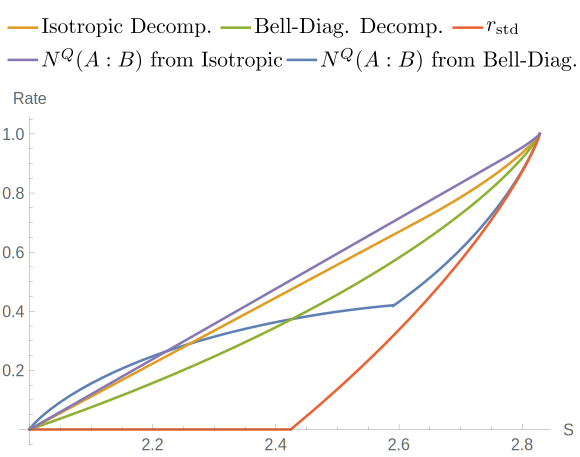
\includegraphics[width=\linewidth]{new_plot.pdf}
        \caption{\label{fig:genubound} Upper bounds based on \Cref{eqn:genubound} for a specific CHSH-based implementation, with either Bell-diagonal states or isotropic states used in the decomposition. The bounds from quantum intrinsic nonlocality~\cite{DIQKD_Limits}, and a bound for the intrinsic nonlocality based on intrinsic information~\cite[Appendix B]{RevisedPeres}, are plotted for comparison. (Source:~\cite{CCSquashedEntangle})}
      \end{figure}

      Let \(\sM\) be a set of POVMs \(\{{\{M_{a|x}\}}_{a}\), \({\{N_{b|y}\}}_{b}\}_{x,y}\), and let \(\cP(\rho, \sM)\) be the behaviour when the state \(\rho = \rho_{Q_A Q_B}\) is measured according to \(\sM\), where we drop the subscripts in this definition. Then, for an arbitrary LOPC protocol, even with two-way information reconciliation, we have~\cite[Thm. 3]{CCSquashedEntangle}
      \begin{equation}\label{eqn:genubound}
        C_{\sk}(p) \leq \inf_{\substack{\rho, \sM : \\ p = \cP(\rho, \sM) }} \inf_{\substack{q : \\ \rho = (1-q)\rho^{NL} + q\rho^L}} (1-q) E_R(\rho^{NL}) + q E_R(\rho^L),
      \end{equation}
      where \(\cP(\rho^L, \sM) \in \Ls\) and \(\cP(\rho^{NL}, \sM) \not\in \Ls\). Essentially, we first select a state and measurement strategy consistent with the observed behaviour, decompose the state into local and nonlocal parts (where states are classified as local or nonlocal based on the chosen measurement strategy), and compute the relative entropy of entanglement for each part.

      While highly general, this bound is extremely difficult to compute, since there are three levels of optimisation that need to be done, including the optimisation for the relative entropy of entanglement. The authors themselves computed this bound only for a specific implementation of the measurements, and specific decompositions of specific states parametrised by CHSH values, as shown in \Cref{fig:genubound}. These are \emph{isotropic states} with
      \begin{equation}
        \rho^{I,v} = (1-v)\ket{\Psi_+}\bra{\Psi_+} + \frac{v}{4}I
      \end{equation}
      and \(S = 2\sqrt{2}(1-v)\), and \emph{Bell diagonal states} with
      \begin{equation}
        \rho^{\Psi,C} = \frac{1+C}{2}\ket{\Psi_+}\bra{\Psi_+} + \frac{1-C}{2}\ket{\Psi_-}\bra{\Psi_-}
      \end{equation}
      and \(S = 2\sqrt{C^2+1}\), where the \emph{Bell states} are
      \begin{equation}
        \ket{\Phi_{\pm}} = \frac{1}{\sqrt{2}}\left( \ket{00} \pm \ket{11} \right) \qquad \ket{\Psi_{\pm}} = \frac{1}{\sqrt{2}}\left( \ket{01} \pm \ket{10} \right).
      \end{equation}
      Fortunately, since all the optimisations are infima, any choice for the parameters is by definition an upper bound, and this bound can be used to evaluate the performance of a protocol on a given implementation.

      The \emph{quantum intrinsic nonlocality} is~\cite{DIQKD_Limits}
      \begin{equation}
        N^Q{(A:B)}_p = \sup_{p(x,y)} \inf_{\rho_{ABXYE}} I{(A:B|XYE)}_{\rho},
      \end{equation}
      where
      \begin{align}
        \rho_{ABXYE} = \sum_{abxy} p(x,y) p(ab|xy) \ket{abxy}\bra{abxy}_{ABXY} \otimes \rho_{E|abxy},
      \end{align}
      with
      \begin{equation}
        p(ab|xy) \rho_{E|abxy} \coloneqq \Tr_{Q_A Q_B}\left[\rho_{Q_A Q_B E} \left(M_{a|x} \otimes N_{b|y} \otimes I_{E}\right) \right]
      \end{equation}
      is Eve's state conditioned on the inputs \(x,y\) and outouts \(a,b\), and \(X\) and \(Y\) being the classical registers holding the values of \(x\) and \(y\). The bound on \(N^Q\) in~\cite{DIQKD_Limits} is outperformed by \Cref{eqn:genubound}, which is in turn outperformed by the bound in~\cite[Appendix B]{RevisedPeres}, but the latter paper restricts itself to protocols that use only one pair of inputs for key generation, and so may not be valid, especially since it is known that using more than one pair of inputs for key generation can improve key rates~\cite{DIQKD_RandomKeyBasis}.

      Unfortunately, all of these bounds are faithful, at least in for the implementations considered. There is thus far only one (possibly) non-faithful upper bound that has been found for quantum adversaries~\cite{NotSufficient}. Interestingly, it uses classical information processing to carry out the attack, by proving the existence of a classical strategy for Eve to reduce the conditional mutual information of Alice and Bob to 0 when certain quantum states are used with any number of measurement settings, if the measurements are projective. However, it applies only to DIQKD protocols where Alice and Bob announce their choice of basis, leaving open the possibility that protocols that do not involve such announcements, such as~\cite{NonstandardProtocol}, may be able to achieve positive key rates, so this is not completely conclusive evidence that \(C_{\sk} = 0\) for these behaviours. However, it seems that this particular protocol has only been proved secure against individual attacks, and it might be interesting to see if it can be proved secure against collective attacks.

      \begin{question}
        What is the key rate of~\cite{NonstandardProtocol} secure against collective attacks?
      \end{question}

      Returning to the bound in~\cite{NotSufficient}, it is known that \emph{Werner states} with visibility \(v\)
      \begin{equation}
        \rho^{W,v} = v{\ket{\Psi_-}\bra{\Psi_-}} + \frac{1-v}{4}I,
      \end{equation}
      cannot exhibit nonlocality for \(v < v_L \approx 0.6829\), but can do so for \(v \geq v_{NL} \approx 0.6964\). However, it is shown that for \(v < v_{\crit} \approx 0.7263 > v_{NL}\), any measurement strategy using projective measurements will produce correlations that can be expressed as a convex combination of behaviours that gives \(I(A:B \downarrow E) = 0\), implying that \(C_{\sk} = 0\) for all such correlations. Since \(v_{NL} < v_{\crit}\), this includes some correlations that exhibit nonlocality. The critical visibility can be increased even further for specific protocols. These behaviours, then, are prospective targets for revival. However, while we are able to specify some behaviours within this set, it is not clear what this set looks like in general. Characterising it might give more insight into how to go about reviving this region.

      \begin{question}
        Can we characterise the quantumly achievable behaviours from Werner states of a given visibility?
      \end{question}

      One version of the \emph{classical-classical (cc) squashed entanglement} defined in~\cite{CCSquashedEntangle} is a convex lower bound to the bound established by this result on Werner state visibilities, as well as the bound in~\cite{RevisedPeres}, while being itself an upper bound for the key rate for the intersection of the sets of applicable protocols for these two results (that is, protocols using Werner states, announcement of basis choice, and only one basis being used for key generation). In particular, it is given by
      \begin{equation}
        E^{cc}_{sq,dev}(\rho, \sM, p(x,y)) = \inf_{\substack{\sigma, \sN : \cP(\sigma, \sN) = \cP(\rho, \sM)}} \sum_{xy} p(x,y) \inf_{\cE_{x,y}} I{(A : B|E)}_{\cE_{x,y}(\psi^{\sigma})},
      \end{equation}
      where \(\cE_{x,y}\) measures \(\psi^\sigma\), the purification of \(\psi^{\sigma}\), using the POVMs in \(\sN\) corresponding to \(x\) and \(y\), while applying an arbitrary CPTP map to Eve's system. Once again, it is fortunate that all optimisations are infima, because this is a difficult optimisation to compute. Although it was applied to bound a specific set of protocols, it might be interesting to see if it could have more general applicability.

      \begin{question}
        What bounds on general protocols can we achieve using the cc-squashed entanglement?
      \end{question}

      \section{Lower Bounds}\label{sec:lbound}

      \subsection{Asymmetric CHSH}

      Instead of using the CHSH inequality directly, it is possible to compute key rates in the standard protocol using asymmetric versions of the CHSH expression
      \begin{equation}
        S_{\alpha} \coloneqq \alpha\angleb{A_0 B_0} + \alpha\angleb{A_1 B_0} + \angleb{A_0 B_1} - \angleb{A_1 B_1}.
      \end{equation}
      This technique can then be combined with noisy preprocessing, where Alice replaces each bit of her key with a locally random bit with probability \(q\). The lower bound for \(H(A|E)\), with \(s = S_{\alpha}\) from the test statistics, is
      \begin{equation} H(A|E) \geq g_{q,\alpha}(s) = \begin{cases}
        g(s) & \text{ for } \abs{\alpha} \geq 1 \text{ or } s \geq s^* \\
        h_2(q) + g'(s^*)(\abs{s}-2) & \text{ otherwise},
      \end{cases}
    \end{equation}
    where
    \begin{equation}
      g_{q,\alpha}(s) = 1 + \phi\left(R_1\right) - \phi\left(R_2\right),
    \end{equation}
    with \(\phi(x) = h_2(1/2 + x/2)\) and
    \begin{equation} 
      R_1 = \sqrt{{(1-2q)}^2 + 4q(1-q)(s^2/4-\alpha^2)} \qquad R_2 = \sqrt{s^2/4-\alpha^2}
    \end{equation}
    and where \(s^*\) is the solution to
    \begin{equation}\label{eqn:sstar}
      h_2(q) + g'(s^*) (s^*-2) = g(s^*).
    \end{equation}

    For a function \(R(s)\) of \(s\), it can easily be verified that
    \begin{equation}
      \diff{\phi(R)}{s} = \frac{1}{2} \diff{R}{s} \log\frac{1-R}{1+R},
    \end{equation}
    and since
    \begin{equation} 
      R_1'(s) = \frac{qs(1-q)}{R_1} \qquad R_2'(s) = \frac{s}{4R_2},
    \end{equation}
    we have
    \begin{equation}\label{eqn:diffg}
      g_{q,\alpha}'(s) = \frac{qs(1-q)}{2R_1} \log\frac{1-R_1}{1+R_1} - \frac{s}{4R_2} \log\frac{1-R_2}{1+R_2}.
    \end{equation}

    The chief difficulty in evaluating this lower bound is optimising the values of \(\alpha\) and \(q\), since the value for \(s^*\) depends on them, but we do not have a closed form expression for it in terms of \(\alpha\) and \(q\). In order to sidestep this issue, we split the problem into three separate optimisations over three parameter regimes, add \(s^*\) as a variable, and enforce \Cref{eqn:diffg} as a constraint where necessary:
    \begin{enumerate}
      \item \(\abs{\alpha} \geq 1\): optimise with \(g_{q,\alpha}(s)\); no need for \(s^*\)
      \item \(\abs{\alpha} \leq 1\) and \(s \leq s^*\): optimise with \(h_2(q) + g'(s^*)(\abs{s}-2)\), constrain \(s^*\) with \Cref{eqn:diffg}
      \item \(\abs{\alpha} \leq 1\) and \(s \geq s^*\): optimise with \(g_{q,\alpha}(s)\), constrain \(s^*\) with \Cref{eqn:diffg}
    \end{enumerate}

    \subsection{Quasi-Relative Entropies}

    A recent approach to lower bounding the secret key uses semidefinite programming to directly compute lower bounds on \(H(A|E)\), by characterising it as a relative entropy
    \begin{equation}
      H{(A|E)}_{\rho} = -D(\rho_{AE}||I_A \otimes \rho_{E}).
    \end{equation}
    Although it does not construct an explicit protocol or implmentation, it is still a useful theoretical tool. 

    As the authors wanted to develop highly general tools that can be used to calculate a variety of quantities and work even for infinite-dimensional cases, they made use of the operator algebra approach to quantum mechanics and spectral theory, which are generally not covered in undergraduate treatments of quantum mechanics and quantum information. Some of these technicalities have been reviewed in \Cref{sec:qretech}, but for our purposes, we can simply focus on the application of these techniques to DIQKD specifically.

    The set of \emph{bounded operators} \(\mathcal{B}(\Hs)\) on the Hilbert space \(\Hs\) is the subset of \(\mathcal{L}(\Hs)\), the set of all linear operators on \(\Hs\), such that the \emph{operator norm} of \(X \in \mathcal{L}(\Hs)\)
      \[ \norm{X} \coloneqq \sup_{\psi \in \Hs \setminus \{0\}} \frac{\norm{X\psi}}{\norm{\psi}} \]
      is finite. Generically, for trace-class operators \(\rho, \sigma \in \mathcal{L}(\Hs)\), where \(\rho \leq \lambda\sigma\) for \(\lambda \in \R^+\),
      \begin{equation}
        D(\rho||\sigma) \leq c_m - \sum_{i=1}^{m-1} \frac{w_i}{t_i \ln 2} \inf_{Z \in \sB(\Hs) : \norm{Z} \leq \alpha_i} \Tr\left[\rho\left(Z + Z^{\dagger}\right)\right] + (1-t_i)\Tr\left[\rho\left(Z^{\dagger}Z\right)\right] + t_i\Tr\left[\sigma\left(ZZ^{\dagger}\right)\right],
      \end{equation}
      where
      \begin{equation}
        c_m = \frac{1}{m^2} \frac{\lambda \Tr[\rho]}{\ln 2} - \sum_{i=1}^m \frac{w_i \Tr[\rho]}{t_i \ln 2} \qquad \alpha_i = \frac{3}{2} \max\left\{\frac{1}{t_i}, \frac{\lambda}{1-t_i}\right\},
      \end{equation}
      and where \(w_i > 0\) and \(t_i \in \ocintv{0}{1}\) are the weights and nodes, respectively, of the \(m\)-point \emph{Gauss-Radau quadrature}, such that \(t_m = 1\), \(w_m = 1/m^2\), and
      \begin{equation}
        \int_{0}^{1} g(t) \dif{t} \approx \sum_{i=1}^m w_i g(t_i),
      \end{equation}
      with equality for all polynomials of degree less than \(2m-2\). Further, the inequality converges to equality as \(m \to \infty\). This quadrature is used to approximate the logarithm, which has the integral representation
      \begin{equation}
        \ln(x) = \int_{0}^{1} \frac{x-1}{t(x-1) + 1} \dif{t},
      \end{equation}
      yielding an approximation in terms of polynomials of operators.

      With \(r\) arbitary linear constraints on the behaviour, indexed by \(j\)
      \[ \sum_{abxy} c^{(j)}_{abxy} p(ab|xy) \geq v_j, \]
      and recalling that
      \[ p(ab|xy) = \Tr\left[\rho_{Q_A Q_B E} \left(M_{a|x} \otimes N_{b|y} \otimes I_{E}\right) \right], \]
      we have the following lower bound on \(H(A|E, X=x^*)\), the conditional entropy for a particular \(x^*\):
      \begin{equation}
        H(A|E, X=x^*) \geq c_m + C_m,
      \end{equation}
      where \(C_m\) is given by
      \begin{align}
        \inf & \sum_{i=1}^{m-1} \frac{w_i}{t_i \ln 2} \sum_a \Tr\left[ \rho_{Q_A Q_B E} \left(M_{a|x^*} \otimes I_{Q_B} \otimes \left( Z_{a,i} + Z_{a,i}^{\dagger} + (1-t_i)  Z_{a,i}^{\dagger}Z_{a,i}\right) \right) + t_i \left( I_{Q_A Q_B} \otimes Z_{a,i}Z_{a,i}^{\dagger}\right)\right] \\
        \text{s.t.} & \begin{aligned}[t] 
          & \sum_{abxy} c^{(j)}_{abxy} \Tr\left[\rho_{Q_A Q_B E} \left(M_{a|x} \otimes N_{b|y} \otimes I_{E}\right) \right] \geq v_j & & \forall 1 \leq j \leq r \\
          & \sum_{a} M_{a|x} = I_{Q_A}, \sum_{b} N_{b|y} = I_{Q_B} & & \forall x, y \\
          & M_{a|x} \geq 0, N_{b|y} \geq 0 & & \forall a, b, x, y \\
          & \norm{Z_{a,i}} \leq \alpha_i & & \forall a, i \in \dintv{1}{m-1} \\
          & M_{a|x} \in \sB(Q_A), N_{b|y} \in \sB(Q_B), Z_{a,i} \in \sB(E) & & \forall a, b, x, y, i \\
          & \rho_{Q_A Q_B E} \text{ is a valid state} & &
        \end{aligned}
      \end{align}

      This optimisation can be converted into an efficiently solvable semidefinite program. By assuming the state of the system on \(Q_A \otimes Q_B \otimes E\) is a pure state \(\ket{\psi}\bra{\psi}_{Q_A Q_B E}\), which can only help Eve (due to data-processing), we can replace all instances of \(\Tr\left[\rho Z\right]\) with \(\braket{\psi|Z\psi}\) for all monomials \(Z\) (individual operators and products of operators, with no operator occuring more than once). These can then be seen as elements of a Gram matrix for the vectors \(Z\ket{\psi}\), which must be positive semidefinite, hence enabling the use of semidefinite programming.

      Finally, in order to constrain \(\rho_{Q_A Q_B E}\) to be a state, we can increase the size of our positive semidefinite matrix by replacing the tensor product structure with a commutation relationship and introducing more terms of the form \(\braket{\psi|\prod M|\psi}\), where \(M \in \{M_{a|x}, N_{b|y}\}\). This is the NPA hierarchy, and in order for the computed Gram matrix to represent a valid quantum strategy, it must be positive semidefinite even with all these terms introduced. The final expression for \(C_m\) then becomes
      \begin{align}
        \inf & \sum_{i=1}^{m-1} \frac{w_i}{t_i \ln 2} \sum_a \bra{\psi} \left(M_{a|x^*} \otimes I_{Q_B} \otimes \left( Z_{a,i} + Z_{a,i}^{\dagger} + (1-t_i)  Z_{a,i}^{\dagger}Z_{a,i}\right) \right) + t_i \left( I_{Q_A Q_B} \otimes Z_{a,i}Z_{a,i}^{\dagger}\right) \ket{\psi} \\
        \text{s.t.} & \begin{aligned}[t] 
          & \sum_{abxy} c^{(j)}_{abxy} \Tr\left[\rho_{Q_A Q_B E} \left(M_{a|x} \otimes N_{b|y} \otimes I_{E}\right) \right] \geq v_j & & \forall 1 \leq j \leq r \\
          & \sum_{a} M_{a|x} = I_{Q_A}, \sum_{b} N_{b|y} = I_{Q_B} & & \forall x, y \\
          & M_{a|x} \geq 0, N_{b|y} \geq 0 & & \forall a, b, x, y \\
          & Z_{a,i} Z_{a,i}^{\dagger} \leq \alpha_i & & \forall a, i \in \dintv{1}{m-1} \\
          & Z_{a,i}^{\dagger} Z_{a,i} \leq \alpha_i & & \forall a, i \in \dintv{1}{m-1} \\
          & M_{a|x}, N_{b|y}, Z_{a,i} \in \in \sB(\Hs) & & \forall a, b, x, y, i \\
          & [M_{a|x}, N_{b|y}] = [M_{a|x}, Z_{b|i}] = [N_{b|y}, Z_{a|i}] = 0 & & \forall a, b, x, y, i \\
          & [M_{a|x}, Z_{b|i}^{\dagger}] = [N_{b|y}, Z_{a|i}^{\dagger}] = 0 & & \forall a, b, x, y, i \\
        \end{aligned}
      \end{align}

      Given the generality of these techniques, one could wonder whether any upper bounds can be computed in this fashion as well. This might help alleviate the optimisation difficulties discussed previously. The quadrature would need to be changed to be an upper bound, rather than a lower bound.
      \begin{question}
        Can any known upper bounds be formulated as quasi-relative entropies and approximated with this method?
      \end{question}

    \section{Nonlocality Monotones}\label{sec:nlmono}

    Instead of trying to find achievable behaviours from a given one, we can try to approach the problem from the opposite direction, by establishing fundamental limits on the achievable behaviours, as was suggessted in \Cref{qn:wirspace}. To this end, we wish to find \emph{monotone measures under wiring}, which are functions of a behaviour that change monotonically when wiring is applied to them. Maximising the key rate over the set of behaviours with the same monotone would then provide an upper bound, and may help give insight into the fundamental limits of wiring.

    In the language of resource theories, monotones are functions that preserve the pre-order of a resource theory~\cite{BellResourceTheory}. That is, for resource \(R_1\) and \(R_2\) in a theory, a monotone \(\mu\) satisfies
    \begin{equation}
      R_1 \leadsto R_2 \Rightarrow \mu(R_1) \geq \mu(R_2).
    \end{equation}
    As mentioned in \Cref{sec:locwir}, wirings are \emph{multiple-copy conversions}~\cite{BellResourceTheory}. Analysis of such conversions has typically consisted of arguments for why specific subsets of \(\NSs\) are or are not closed under wiring, for example by constructing explicit wirings that convert a behaviour in the set to one that is outside the set~\cite{ClosedCorrSets} or by arguments from the structure of the set to show that the set must be closed under wirings~\cite{NonlocalZoo}. Indeed, we were able to find only one reference,~\cite{NLMonotones}, providing concrete measures that are explicitly proved to be monotone under wirings under a set of free actions that is a strict superset of \(\sW_D\) defined in \Cref{sec:locwir}. These wirings additionally allow the order in which the boxes are used to be permuted and for non-deterministic wirings. However, its monotonicity under wirings with shared randomness was not proved. Nonetheless, we will review these results to see how they can help us.

    \subsection{Maximal Correlation and Related Measures}\label{sec:nlmono_maxcorr}

    The maximal correlation between two random variables (rvs) \(A,B\) is denoted as \(\rho(A,B)\) and defined as~\cite{NLMonotones}
    \begin{equation}
      \rho(A,B) = \max_{f,g} \frac{\E[(f(A)-\E[f(A)])(g(B)-\E[g(B)])]}{\sqrt{\Var[f(A)]\Var[g(B)]}}
    \end{equation}
    or equivalently
    \begin{Array}{rcl}
      \rho(A,B) = & \max_{f,g}  & \E[f(A)g(B)] \\
                  & \text{s.t.} & \E[f(A)] = \E[g(B)] = 0 \\
                  &             & \E[f(A)^2] = \E[g(B)^2] = 1,
    \end{Array}
    where the equivalent description essentially enforces normalisation on the functions to simplify the expression.

    The maximal correlation is a nonlocality monotone because it possesses the \emph{tensorisation} property: if rvs \((A_1, B_1)\) are statistically independent of \((A_2,B_2)\), that is, their pmfs obey \(P_{A_1A_2B_1B_2} = P_{A_1B_1}P_{A_2B_2}\), then
    \begin{equation}
      \rho(A_1A_2,B_1B_2) = \max\{ \rho(A_1,B_1), \rho(A_2,B_2) \}.
    \end{equation}
    In particular, this means that the maximal correlation of \(n\) i.i.d.\ copies of the pair \((A,B)\) is \(\rho(A,B)\), even though the functions \(f\) and \(g\) can operate on all copies at once. This seems to imply that wiring cannot increase the maximal correlation between \(A\) and \(B\).

    To apply it more formally to wirings, we define \(\rho(A,B|X=x,Y=y)\) as the maximal correlation computed using the distribution \(P_{AB}(a,b) = p(ab|xy)\). If we wire the bxoes that Alice used in over several rounds together, and did likewise with Bob, the boxes in each round can be seen as having a joint distribution determined by \((x,y)\). Although the choice of \((x,y)\) in each round is no longer independent of the previous rounds, the distributions conditioned on \((x,y)\) are still independent. Therefore, the maximal correlation of the boxes that are wired together cannot exceed
    \[ \max_{x,y} \rho(A,B|X=x,Y=y). \]
    Since the output rvs \(A', B'\) after wiring are themselves functions of the rvs corresponding to the individual rounds, this can only restrict the possible range of \(f\) and \(g\) when computing their maximal correlation, as compared to the maximal correlation of the individual rounds. Therefore
    \[ \rho(A',B'|X=x,Y=y) \leq \max_{x,y} \rho(A,B|X=x,Y=y). \]

    The maximal correlation is particularly important because it can be efficiently computed given a distribution, despite its generality. We define the matrices
    \begin{align}
      \matrp{P}{_{AB|xy}}_{ab} &= \Pr(A = a, B = b|X = x, Y = y) \\
      \matrp{P}{_{A|x}}_{ab} &= \delta_{ab} \Pr(A = a|X = x) \\
      \matrp{P}{_{B|y}}_{ab} &= \delta_{ab} \Pr(B = b|Y = y) \\
      \matrp{\tilde{P}}{_{AB|xy}} &= \matrp{P}{_{A|x}}^{-1/2} \matrp{P}{_{AB|xy}} \matrp{P}{_{B|y}}^{-1/2} \\
      \therefore \matrp{\tilde{P}}{_{AB|xy}}_{ab} &= \frac{p(a,b|x,y)}{\sqrt{p(a|x)p(b|y)}},
    \end{align}
    where \(\matrp{P}{_{A|x}}_{ab}\), \(\matrp{P}{_{B|y}}_{ab}\), \(\matrp{P}{_{AB|xy}}_{ab}\) and \(\matrp{\tilde{P}}{_{AB|xy}}\) have dimensions \(o_A \times o_A\), \(o_B \times o_B\), \(o_A \times o_B\), \(o_A \times o_B\) respectively. We use the Moore-Penrose inverse for this inversion, which, since \(\matrp{P}{_{A|x}}_{ab}\) and \(\matrp{P}{_{B|y}}_{ab}\) are diagonal, involves inverting their non-zero diagonal entries and leaving the zero entries in place.

    Let the singular values of \(\matrp{\tilde{P}}{_{AB|xy}}\) be \(\sigma_i\) for \(i \in \dintv{1}{\min\{o_A, o_B\}}\) such that \(\sigma_{i} \geq \sigma_{i+1}\),
    \begin{equation}
      \rho(A,B|X=x,Y=y) = \sigma_2\left( \matrp{\tilde{P}}{_{AB|xy}} \right).
    \end{equation}

    Working with the normalised form of the maximum correlation function, and so considering only normalised functions, we have
    \begin{align}
      \E[f(A)g(B)|xy] &= \sum_{a,b} p(a,b|x,y) f(a)g(b) \\
                      &= \sum_{a,b} \sqrt{p(a|x)} f(a) \frac{p(a,b|x,y)}{\sqrt{p(a|x)p(b|y)}} \sqrt{p(b|y)} g(b) \\
                      &= \rvec{f} \matrp{\tilde{P}}{_{AB|xy}} \cvec{g},
    \end{align}
    where we have defined
    \begin{equation}
      \cvec{f} = {[\sqrt{p(a|x)} f(a)]}^T_a \qquad \cvec{g} = {[\sqrt{p(b|y)} g(b)]}^T_b.
    \end{equation}
    The technicalities arising from cases where \(p(a|x)\) or \(p(b|y)\) are zero, which result in \(p(a,b|x,y)\) being divided by zero, are handled by the Moore-Penrose inverse, which maps those entries of \(\matrp{\tilde{P}}{_{AB|xy}}\) to zero.

    We also represent \(\matrp{\tilde{P}}{_{AB|xy}}\) in its compact singular value decomposition as
    \begin{equation}
      \matrp{\tilde{P}}{_{AB|xy}} = \sum_i \sigma_i \cvec{u}_i \rvec{v}_i,
    \end{equation}
    where \(\{\cvec{u}_i\}\) and \(\{\cvec{v}_i\}\) are sets of orthonormal vectors in \(\R^{o_A}\) and \(\R^{o_B}\) respectively.

    It is known that~\cite[Thm 1]{ComputingMaxCorr} \(\sigma_i \in [0, 1]\), and
    \begin{equation}
      \sigma_1 = 1 \qquad \cvec{u}_1 = {[\sqrt{p(a|x)}]}_a^T \qquad \cvec{v}_1 = {[\sqrt{p(b|y)}]}_b^T.
    \end{equation}
    This gives us that
    \begin{align}
      \rvec{f} \cvec{u}_1 &= \sum_a p(a|x) f(a) = \E[f(A)|x] = 0 \\
      \norm{\cvec{f}}_2 &= \sum_a p(a|x) {f(a)}^2 = \E[{f(A)}^2|x] = 1 \\
      \rvec{v}_1 \cvec{g} &= \sum_b p(b|y) g(b) = \E[g(B)|y] = 0 \\
      \norm{\cvec{g}}_2 &= \sum_b p(b|y) {g(b)}^2 = \E[{g(B)}^2|y] = 1.
    \end{align}

    The singular value decomposition can be characterised variationally by
    \begin{Array}{rcl}
      \sigma_1(\matr{M}) = & \max_{\cvec{f},\cvec{g}} & \rvec{f} \matr{M} \cvec{g} \\
                            & \text{s.t.} & \norm{\cvec{f}}_2 = \norm{\cvec{g}}_2 = 1, \\
    \end{Array}
    for an arbitrary matrix \(\matr{M}\) by using Lagrange multipliers to constrain \(\cvec{f}\) and \(\cvec{g}\). This maximum is achieved by \(\cvec{f} = \cvec{u}_1\), \(\cvec{g} = \cvec{v}_1\). With the additional constraint of \(\rvec{f} \cvec{u}_1 = \rvec{v}_1 \cvec{g} = 0\), the maximum is \(\sigma_2(\matr{M})\), achieved by \(\cvec{f} = \cvec{u}_2\), \(\cvec{g} = \cvec{v}_2\). We can apply this property directly to find the maximal correlation, and the functions which achieve it, from the singular value and corresponding singular vectors for \(i = 2\).

    In~\cite{NLMonotones}, these properties of the maximal correlation are proved using the properties of various related measures, that typically take the form of \emph{ribbons}: subsets of \({[0,1]}^2\). These include the hypercontractivity (HC) ribbon:
    \begin{equation}
      \HC(A,B) = \{(\nu_A, \nu_B) \in {[0,1]}^2 \st \forall U, \nu_A I(U:A) + \nu_B I(U:B) \leq I(U:AB)\},
    \end{equation}
    or equivalently,
    \begin{equation}
      \HC(A,B) = \{(\nu_A, \nu_B) \in {[0,1]}^2 \st \forall f,g; \E[f(A)g(B)] \leq {\E[\abs{f(A)}^{1/\nu_A}]}^{\nu_A} {\E[\abs{g(B)}^{1/\nu_B}]}^{\nu_B} \},
    \end{equation}
    or, with \(\Upsilon_{AB}(\nu_A, \nu_B) = \nu_A H(A) + \nu_B H(B) - H(AB)\) and \(\tilde{\Upsilon}_{AB}\) its lower convex envelope (pointwise largest convex function that fulfills \(\tilde{\Upsilon}_{AB}(\nu_A, \nu_B) \leq \Upsilon_{AB}(\nu_A, \nu_B)\) for all \(\nu_A, \nu_B\)):
    \begin{equation}
      \HC(A,B) = \{(\nu_A, \nu_B) \in {[0,1]}^2 \st \Upsilon_{AB}(\nu_A, \nu_B) = \tilde{\Upsilon}_{AB}(\nu_A, \nu_B) \};
    \end{equation}
    and the maximal correlation (MC) ribbon:
    \begin{equation}
      \MC(A,B) = \left\{ 
        (\nu_A, \nu_B) \in {[0,1]}^2 \st \forall f; \Var[f(A,B)] \geq 
        \begin{aligned}[c]
          & \nu_A \Var_A[\E_{B|A}[f(A,B)]] \\
          + & \nu_B \Var_B[\E_{A|B}[f(A,B)]] \\
        \end{aligned}
      \right\},
    \end{equation}
    which can be normalised by restricting to \(\E[f(A,B)] = 0\), giving
    \begin{equation}
      \MC(A,B) = \left\{(\nu_A, \nu_B) \in {[0,1]}^2 \st \forall f; \E[{f(A,B)}^2] \geq 
        \begin{aligned}[c]
          & \nu_A \E_A[{(\E_{B|A}[f(A,B)])}^2] \\ + & \nu_B \E_B[{(\E_{A|B}[f(A,B)])}^2] \\
        \end{aligned}
      \right\}.
    \end{equation}

    The ribbon for a behaviour can be defined as the intersection of the ribbons for the individual conditional distributions. The ribbons have the tensorisation property, the ribbon of a post-wiring behaviour is a superset of the intersection of the ribbon of pre-wiring behaviours (that is, it expands under wirings), and the ribbons occupy the whole of \({[0,1]}^2\) for independent variables, while being restricted to \(\{(\nu_A, \nu_B) \st \nu_A + \nu_B \leq 1\}\) for perfectly correlated boxes. This makes them nonlocality monotones in the sense of monotonically changing under wirings, despite not fulfilling the resource-theoretic definition since they are not scalars.

    The relations between the measures discussed are
    \begin{gather}
      {\rho(A,B)}^2 = \inf_{\substack{(\nu_A, \nu_B) \in \MC(A,B) \\ \nu_B \neq 0}} \frac{1 - \nu_A}{\nu_B} \\
      \HC(A,B) \subseteq \MC(A,B) \\
      s^*(A,B) \coloneqq \inf_{\substack{(\nu_A, \nu_B) \in \HC(A,B) \\ \nu_B \neq 0}} \frac{1 - \nu_A}{\nu_B} \geq {\rho(A,B)}^2
    \end{gather}

    \subsection{CHSH Distillability of Isotropic Boxes}\label{sec:nlmono_isodist}

    In this work, it was proved that wirings without shared randomness cannot distill one isotropic box to another with a larger violation of CHSH. The case with shared randomness was proved for boxes with a PR fraction in \([1/\sqrt{2}, 1]\), which is precisely the part of the isotropic line outside of \(\Qs\). A crucial step of the proof was to show that isotropic boxes have the lowest maximal correlation of all boxes with a given CHSH value, the proof of which relied only worked for superquantum values of the PR fraction.

    Nonetheless, if we could characterise the impact of shared randomness on the maximal correlation, this part of the proof could be completed, since there does exist a wiring that uses shared randomness to turn any box into an isotropic box with the same CHSH value~\cite{NSTheories}. If we can show that wirings using shared randomness do not increase the maximal correlation, then we will be able to prove that isotropic boxes are not distillable, while also proving that maximal correlation is a monotone under \(\sW\), not just for \(\sW_D\).

    \begin{question}
      How does the use of shared randomness in wirings affect the maximal correlation and other related measures?
    \end{question}

    \subsection{Evaluation}

    The ideal nonlocality monotone \(\mu\) would have the following desiderata:
    \begin{enumerate}
      \item Given a behaviour \(p\), it is easy to compute \(\mu(p)\)
      \item Given a value \(\mu'\), the set \(\{ p \st \mu(p) = \mu' \}\), the set can be efficiently optimised over
      \item It is tight in the sense that if \(\mu(p) = \mu(p')\) for behaviours \(p\) and \(p'\), there exists a wiring that will transform \(p \mapsto p'\)
      \item Given \(p\) and \(p'\), if \(\mu(p) = \mu(p')\), we can expicitly construct the wiring that transforms \(p\) into \(p'\)
    \end{enumerate}

    Property 1 is satisfied by the maximal correlation, but the extent to which it satisfies the other desiderata is still unclear. However, given that its monotonicity is derived from that of higher-dimensional monotones, namely the MC and HC ribbons, it is unlikely that the maximal correlation is tight (Property 3), since a transformation could change other regions of the ribbon without affecting the maximal correlation. Nonetheless, it would be helpful to see if these measures can satisfy these demands, or to find out why it might not be possible to meet them.

    Another caveat arises when attempting to explicitly compute bounds on the key rate from the maximal correlation. Observe that, for \(K_A\) and \(K_B\), two perfectly correlated and uniformly distributed secret keys, we have \(\rho(K_A, K_B) = 1\), with the maximum achieved by mapping half of the keys to \(1\) and half to \(-1\) for both \(f\) and \(g\). However, if the two keys are independent, then \(\rho(K_A,K_B) = \E[f(K_A)g(K_B)] = \E[f(K_A)]\E[g(K_B)] = 0\). Likewise, if the two keys are deterministic (not secret), then \(f(K_A) = g(K_B) = 0\) and so \(\rho(K_A, K_B) = 0\). However, this poses an issue for longer keys. As long as \(K_A\) and \(K_B\) are uniformly distributed over \(N > 1\) values, \(\rho(K_A, K_B) = 1\), regardless of whether \(N = 2\) or (say) \(N = 10^{12}\). Therefore, we need to find a bound that looks something like
    \begin{equation}
      \max_{E|AB} \frac{H(A|E) - H(A|B)}{H(A)} \leq f(\rho(A,B))
    \end{equation}
    in order to achieve the correct scaling for an estimate of the key rate.

    \section{Summary and Outlook}

    The study of distillation via wiring multiple boxes together has largely fallen by the wayside, and there has been little attention paid to the idea in DIQKD research. However, this review has uncovered a vast variety of related tools and approaches for tackling this problem, for studying the space of behaviours, the space of wirings, and upper and lower bounds on key rates. Having consolidated these techniques, we are ready to embark on a deeper and more focused attempt to apply them. We hope that we will be able to uncover some interesting insights about the structure of nonlocality by utilising these different approaches and techniques.

    \printbibliography{}

    \begin{appendices}
      \section{Technicalities for Quasi-Relative Entropies}\label{sec:qretech}

      For an operator \(A \in \mathcal{L}(\Hs)\), its \emph{spectrum} \(\sigma(A)\) is the subset of \(\C\) such that, for all \(\lambda \in \sigma(A)\), \(A - \lambda I\) does not have a \emph{bounded inverse}: there does not exist an operator \(S\) such that \(S\left( A - \lambda I \right) = \left( A - \lambda I \right)S =  I\) and \(S \in \mathcal{B}(\Hs)\).

      Our objective is to establish a \emph{functional calculus} that will allow us to evaluate a function  \(f\) with scalar output on operators. In the finite-dimensional case this is straightforward for normal operators (obeying \(AA^{\dagger} = A^{\dagger}A\)): for an operator \(A\) with eigenvalues \(\{\lambda_i\}\) and corresponding eigenprojectors \(\{\Pi_i\}\),
      \[ A = \sum_i \lambda_i \Pi_i \Rightarrow f(A) = \sum_i f(\lambda_i) \Pi_i, \]
      by the \emph{spectral theorem}.

      However, the approach of the paper generalises the spectral theorem to cases where the spectrum \(\sigma(A)\) is no longer a discrete set of eigenvalues, as it is in the finite-dimensional case, but a \emph{continuous spectrum}. This scenario arises in infinite-dimensional Hilbert spaces, such as those involving position and momentum operators. These particular operators are even more complex, since they are \emph{unbounded}. We will therefore sketch the standard statement of the spectral theorem, which applies to bounded normal operators and unbounded self-adjoint (\(A = A^{\dagger}\)) operators, although we leave aside technicalities regarding the domain of the operators and the functions involved in this generalisation.

      This requires some additional definitions. \emph{Spectral measures}, or \emph{projector-valued measures} (PVMs), map a subset of the spectrum to a projector. More formally, they are functions between the \emph{\(\sigma\)-algebra} \(\Omega(\sigma(A))\) of \(\sigma(A)\) to \(\mathcal{B}(\Hs)\). A \(\sigma\)-algebra contains subsets of its underlying set, and is closed under set complements and unions of countable sequences, so in this case it represents subsets of the spectrum that it would be sensible to attach a projector to.

      In the finite-dimensional case, the projector associated to each eigenvalue \(\lambda\) in the spectrum is the projector onto the associated eigenspace, and the direct sum of the projectors is the projector onto \(\Hs\), that is, \(I\). With a continuous spectrum, we want to divide \(\Hs\) into orthogonal spaces in the same way, providing a systematic way to attach each subspace to each element \(\omega \in \Omega(\sigma(A))\), that is, each reasonable subset of \(\sigma(A)\). Under a given spectral measure \(E : \Omega(\sigma(A)) \to \mathcal{B}(\Hs)\), the subspace \(V_{\omega} \subseteq \Hs\) associated to \(\omega\) is called a \emph{spectral subspace}, and \(E(\omega)\) is the projector onto \(V_{\omega}\). These \(V_{\omega}\) are ``generalised eigenspaces'' in the sense that they are \emph{invariant} under \(A\), that is, \(\psi \in V_{\omega} \Rightarrow A\psi \in V_{\omega}\), and that, for \(\omega \subseteq [\lambda - \epsilon, \lambda + \epsilon]\), we have \(\norm{(A - \lambda I)\psi} \leq \epsilon\norm{\psi}\), from which recover the familiar behaviour when the spectrum is discrete.

      A function \(f : \sigma(A) \to \C\) can then be applied to an element of \(\mathcal{B}(\Hs)\), by integrating it against this measure
      \[ f(A) = \int_{\lambda \in \sigma(A)} f(\lambda) \dif{E(\lambda)}, \]
      where we have that
      \[ \int_{\lambda \in \sigma(A)} \delta\{\lambda \in \omega\} \dif{E(\lambda)} = E(\omega), \]
      with the \emph{indicator function} \(\delta\{P\} = 1\) when \(P\) is true, and 0 otherwise. This property can be used to define the integral for any other function. For example, for a given function \(f : \R \to \C\), we can define a sequence of functions
      \[ f_n(\lambda) = \sum_{j = -\infty}^{\infty} f(j/n) \delta\{\lambda \in [j/n, (j+1)/n)\}, \]
      and if this sequence \emph{converges uniformly} to \(f(\lambda)\), that is,
      \[ \forall \lambda \in \C; \lim_{n \to \infty} \norm{f_n(\lambda) - f(\lambda)} = 0, \]
      then
      \[ f(A) = \lim_{n\to\infty} \int_{\lambda \in \sigma(A)} f_n(\lambda) \dif{E(\lambda)} = \lim_{n\to\infty} \sum_{j = -\infty}^{\infty} f(j/n) E([j/n, (j+1)/n)) \]
      so that, roughly speaking, the effect of \(f(A)\) on \(E([\lambda, \lambda+\dif{\lambda}))\psi\) is multiplication by \(f(\lambda)\). The \emph{spectral theorem} then asserts that there is a \emph{unique} measure \(E_A\) on the Borel \(\sigma\)-algebra, that is, the smallest \(\sigma\)-algebra containing all open sets in \(\sigma(A)\), such that
      \[ A = \int_{\sigma(A)} \lambda \dif{E_A(\lambda)}, \]
      which is how \(A\) can be decomposed into orthogonal projectors.

      An operator-valued measure \(E\) on \(\sigma(A)\) can be converted into a regular, scalar-valued measure \(\nu\) by specifying a vector \(\phi\), so that
      \[ \int_{\sigma(A)} f(\lambda) \dif{\nu(\lambda)} = \angleb{\phi, \left(\int_{\sigma(A)} f(\lambda) \dif{E(\lambda)}\right) \phi}. \]

      A \emph{joint spectral measure} of multiple self-adjoint operators, with \emph{commuting spectral measures} (which then implies that the operators commute) is then simply the product of their respective spectral measures, with a straightforward generalisation from the single-operator case.

      % TODO replace \sigma(A) with \mathcal{X} and explain the use of joint spectral
      % measures in the paper

    \end{appendices}

    \end{document}

    Compute relative entropy of entanglement and compare to quantum maximal correlation
